
\documentclass[working, openany]{tuftebook}

\usepackage{afterpage}

\usepackage[utf8]{inputenc}
\usepackage[T1]{fontenc}
\usepackage{textcomp}

\usepackage{pdfpages}
\usepackage{lipsum}
\usepackage{parskip}
\usepackage{titletoc}
\usepackage{svg}

% \usepackage{vub}

\usepackage{url}
\usepackage[backend=biber,
style=authoryear,
uniquename=false,
uniquelist=false,
citestyle=authoryear,
dashed=false]{biblatex}
\addbibresource{references.bib}
\renewcommand*{\nameyeardelim}{\addcomma\space}

\usepackage{hyperref}
\hypersetup{
    colorlinks,
    linkcolor={black},
    citecolor={black},
    urlcolor={blue!80!black}
}
\usepackage[noabbrev]{cleveref}

\setlength\bibitemsep{1.5\itemsep}


\AtEveryBibitem{
    \clearfield{urlyear}
    \clearfield{urlmonth}
    \clearfield{month}
    \clearlist{language}
    % \clearfield{doi}
    \clearfield{issn}
    % \clearfield{isbn}
    \clearfield{url}
}

% Adds Bibliography, ... to Table of Contents
\usepackage[nottoc]{tocbibind}

\usepackage{graphicx}
\usepackage{float}
% \usepackage[usenames,dvipsnames,svgnames]{xcolor}
% \usepackage{cmbright}




\usepackage{amsmath, amsfonts, mathtools, amsthm, amssymb}
\usepackage{mathrsfs}
\usepackage{cancel}

\newcommand\N{\ensuremath{\mathbb{N}}}
\newcommand\R{\ensuremath{\mathbb{R}}}
\newcommand\Z{\ensuremath{\mathbb{Z}}}
\renewcommand\O{\ensuremath{\emptyset}}
\newcommand\Q{\ensuremath{\mathbb{Q}}}
\newcommand\C{\ensuremath{\mathbb{C}}}
\let\implies\Rightarrow
\let\impliedby\Leftarrow
\let\iff\Leftrightarrow
\let\epsilon\varepsilon

\usepackage{tikz}
\usepackage{tikz-cd}

% theorems
\usepackage{thmtools}
\usepackage{thm-restate}
\usepackage[framemethod=TikZ]{mdframed}
\mdfsetup{skipabove=1em,skipbelow=0em, innertopmargin=12pt, innerbottommargin=8pt}



\theoremstyle{definition}

\makeatletter

\declaretheoremstyle[headfont=\bfseries\sffamily, bodyfont=\normalfont, mdframed={ nobreak } ]{thmgreenbox}
\declaretheoremstyle[headfont=\bfseries\sffamily, bodyfont=\normalfont, mdframed={ nobreak } ]{thmredbox}
\declaretheoremstyle[headfont=\bfseries\sffamily, bodyfont=\normalfont]{thmbluebox}
\declaretheoremstyle[headfont=\bfseries\sffamily, bodyfont=\normalfont]{thmblueline}
\declaretheoremstyle[headfont=\bfseries\sffamily, bodyfont=\normalfont, numbered=no, mdframed={ rightline=false, topline=false, bottomline=false, }, qed=\qedsymbol ]{thmproofbox}
\declaretheoremstyle[headfont=\bfseries\sffamily, bodyfont=\normalfont, numbered=no, mdframed={ nobreak, rightline=false, topline=false, bottomline=false } ]{thmexplanationbox}

\declaretheoremstyle[headfont=\bfseries\sffamily, bodyfont=\normalfont, numbered=no, mdframed={ nobreak, rightline=false, topline=false, bottomline=false } ]{thmexplanationbox}


\declaretheorem[numberwithin=chapter, style=thmgreenbox, name=Definition]{definition}
\declaretheorem[sibling=definition, style=thmredbox, name=Corollary]{corollary}
\declaretheorem[sibling=definition, style=thmredbox, name=Proposition]{prop}
\declaretheorem[sibling=definition, style=thmredbox, name=Theorem]{theorem}
\declaretheorem[sibling=definition, style=thmredbox, name=Lemma]{lemma}
\declaretheorem[sibling=definition, style=thmbluebox,  name=Example]{eg}
\declaretheorem[sibling=definition, style=thmbluebox,  name=Nonexample]{noneg}
\declaretheorem[sibling=definition, style=thmblueline, name=Remark]{remark}



\declaretheorem[numbered=no, style=thmexplanationbox, name=Proof]{explanation}
\declaretheorem[numbered=no, style=thmproofbox, name=Proof]{replacementproof}
\declaretheorem[style=thmbluebox,  numbered=no, name=Exercise]{ex}
\declaretheorem[style=thmblueline, numbered=no, name=Note]{note}

% \renewenvironment{proof}[1][\proofname]{\begin{replacementproof}}{\end{replacementproof}}

% \AtEndEnvironment{eg}{\null\hfill$\diamond$}%

\newtheorem*{uovt}{UOVT}
\newtheorem*{notation}{Notation}
\newtheorem*{previouslyseen}{As previously seen}
\newtheorem*{problem}{Problem}
\newtheorem*{observe}{Observe}
\newtheorem*{property}{Property}
\newtheorem*{intuition}{Intuition}


\declaretheoremstyle[
    headfont=\bfseries\sffamily\color{RawSienna!70!black}, bodyfont=\normalfont,
    mdframed={
        linewidth=2pt,
        rightline=false, topline=false, bottomline=false,
        linecolor=RawSienna, backgroundcolor=RawSienna!5,
    }
]{todo}
\declaretheorem[numbered=no, style=todo, name=TODO]{TODO}


\usepackage{etoolbox}
\AtEndEnvironment{vb}{\null\hfill$\diamond$}%
\AtEndEnvironment{intermezzo}{\null\hfill$\diamond$}%

% http://tex.stackexchange.com/questions/22119/how-can-i-change-the-spacing-before-theorems-with-amsthm
\def\thm@space@setup{%
  \thm@preskip=\parskip \thm@postskip=0pt
}

\usepackage{xifthen}

\makeatother

% figure support (https://castel.dev/post/lecture-notes-2)
\usepackage{import}
\usepackage{xifthen}
\pdfminorversion=7
\usepackage{pdfpages}
\usepackage{transparent}


\makeatletter
\newif\ifworking
\@ifclasswith{tuftebook}{working}{\workingtrue}{\workingfalse}
\makeatother

\newcommand{\incfig}[2][1]{%
    % \ifworking{\makebox[0pt][c]{\color{gray}{\scriptsize\textsf{#2}}}}\fi%
    \def\svgwidth{#1\textwidth}
    \import{./figures/}{#2.pdf_tex}
}

\newcommand{\fullwidthincfig}[2][0.90]{%
    % \ifworking{\makebox[0pt][l]{\color{gray}{\scriptsize\textsf{#2}}}}\fi%
    \def\svgwidth{#1\paperwidth}
    \import{./figures/}{#2.pdf_tex}
}



\newcommand{\minifig}[2]{%
    \def\svgwidth{#1}%
    \begingroup%
    \setbox0=\hbox{\import{./figures/}{#2.pdf_tex}}%
    \parbox{\wd0}{\box0}\endgroup%
    \hspace*{0.2cm}
}





% %http://tex.stackexchange.com/questions/76273/multiple-pdfs-with-page-group-included-in-a-single-page-warning
\pdfsuppresswarningpagegroup=1

\newcommand\todo[1]{\ifworking {{\color{red}{#1}}} \else {}\fi}

\author{Anastasia Krouglova}



\usepackage{multirow}
\def\block(#1,#2)#3{\multicolumn{#2}{c}{\multirow{#1}{*}{$ #3 $}}}

% \overfullrule=1mm

\newenvironment{myproof}[1][\proofname]{%
  \proof[\rm \bf #1]%
}{\endproof}

% Author: Izaak Neutelings (January 2021)
% http://pgfplots.net/tikz/examples/fourier-transform/
% https://tex.stackexchange.com/questions/127375/replicate-the-fourier-transform-time-frequency-domains-correspondence-illustrati
% https://www.dspguide.com/ch13/4.htm
\usepackage{amsmath}
\usepackage{tikz}
\usepackage{physics}
\usepackage[outline]{contour} % glow around text
\usepackage{xcolor}
\usetikzlibrary{intersections}
\usetikzlibrary{decorations.markings}
\usetikzlibrary{angles,quotes} % for pic
\usetikzlibrary{calc}
\usetikzlibrary{3d}
\contourlength{1.3pt}

\tikzset{>=latex} % for LaTeX arrow head


\definecolor{mygrey}{RGB}{167,192,224}

\definecolor{mybluegrey}{RGB}{120, 150, 184}
\definecolor{mycyangrey}{RGB}{137,190,198}


\definecolor{bluesquare}{RGB}{213,232,255}
\definecolor{cyansquare}{RGB}{193,234,241}

\definecolor{bluecontour}{RGB}{242,248,255}


\definecolor{myblue}{RGB}{0,0,166}
\definecolor{mycyan}{RGB}{167,192,224}
\definecolor{mygreen}{RGB}{167,192,224}
\definecolor{myorange}{RGB}{167,192,224}
\definecolor{myred}{RGB}{239,85,59}
\definecolor{mydarkred}{RGB}{167,192,224}
\definecolor{mypurple}{RGB}{167,192,224}
\colorlet{mydarkblue}{myblue!80!black}

% \colorlet{myred}{red!85!black}
% \colorlet{myorange}{orange!90!black!80}
% \colorlet{mydarkred}{myred!80!black}
\tikzstyle{xline}=[myblue,thick]
\def\tick#1#2{\draw[thick] (#1) ++ (#2:0.1) --++ (#2-180:0.2)}
\tikzstyle{myarr}=[myblue!50,-{Latex[length=3,width=2]}]
\def\N{90}




% SQUARE WAVE 
\def\xmin{-0.7*\T}   % min x axis
\def\xmax{6.0}       % max x axis
\def\ymin{-1.04}     % min y axis
\def\ymax{1.3}       % max y axis
\def\A{0.67*\ymax}   % amplitude
\def\T{(0.35*\xmax)} % period
\def\f#1{\A*4/pi/(#1)*sin(360/\T*#1*Mod(\t,\T))} 

% SYNTHESIS 3D
\newcommand{\tikzFourierTransform}[1]{
\begin{tikzpicture}[x=(-20:0.9), y=(90:0.9), z=(42:1.1)]
  \message{^^JSynthesis 3D}
  \def\xmax{6.5}        % max x axis
  \def\ymin{-1.2}       % min y axis
  \def\ymax{1.6}        % max y axis
  \def\zmax{5.8}        % max z axis
  \def\xf{1.17*\xmax}   % x position frequency axis
  \def\A{(0.60*\ymax)}  % amplitude
  \def\T{(0.335*\xmax)} % period
  \def\w{\zmax/11.2}    % spacing components
  
  % COMPONENTS
  \foreach \i/\col [evaluate={\z=\w*\i;}] in {
      11/mycyan,9/mypurple,7/myorange,5/myred,3/mygreen,1/mygrey}{
    \draw[black!30] ({\T},0.1,\z) --++ (0,-0.2,0);
    \draw[black!30] ({2*\T},0.1,\z) --++ (0,-0.2,0);
    \draw[->,black!30] (0,0,\z) --++ (0.93*\xmax,0,0);
    \draw[xline,\col,opacity=0.8,thick,
          samples=\i*\N,smooth,variable=\t,domain=-0.05*\T:0.87*\xmax]
      plot(\t,{\f{\i}},\z);
  }
  
  % TIME DOMAIN
  \begin{scope}[shift={(0,0,-0.17*\zmax)}]
    \draw[bluesquare,fill=bluesquare,opacity=0.4,canvas is xy plane at z=0]
      (-0.1*\xmax,-1.25*\ymax) rectangle (1.13*\xmax,1.25*\ymax);
    \draw[->,mybluegrey,thick] (-0.05*\xmax,0,0) -- (\xmax,0,0)
      node[below right=-3,canvas is xy plane at z=0] {$t$ [s]};
    \draw[->,mybluegrey,thick] (0,\ymin,0) -- (0,\ymax,0)
      node[left,canvas is xy plane at z=0] {$y$};
    \draw[xline,myblue,thick,
          samples=9*\N,smooth,variable=\t,domain=-0.05*\T:0.9*\xmax]
      plot(\t,{\f{1}+\f{3}+\f{5}+\f{7}+\f{9}+\f{11}},0); %node[above] {$f$};
    \tick{{\T},0,0}{90}
      node[below=-1,scale=0.9,canvas is xy plane at z=0] {\contour{bluecontour}{$T$}};
    \tick{{2*\T},0,0}{90}
      node[below=-1,scale=0.9,canvas is xy plane at z=0] {\contour{bluecontour}{$2T$}};
    \node[scale=1,canvas is xy plane at z=0] at (0.4*\xmax,-\ymax,0) {Time domain};
  \end{scope}
  
  % FREQUENCY DOMAIN
  \begin{scope}[shift={(\xf,0,0)}]
    \draw[cyansquare,fill=cyansquare,opacity=0.3,canvas is zy plane at x=0]
      (-0.13*\zmax,-1.25*\ymax) rectangle (1.26*\zmax,1.25*\ymax);
    %\draw[->,thick] (0,0,0) -- (0,0,\zmax) node[above left=-1] {$z$};
    %\draw[->,thick] (\xmax,0,0) --++ (0,0,\zmax);
    \draw[->,mycyangrey,thick] (0,0.8*\ymin,0) -- (0,\ymax,0)
      node[above=2,left=0,canvas is zy plane at x=0] {$a_n$};
      %node[pos=0.84,left=2,fill=white,inner sep=0] {$b_n$};
    \draw[->,mycyangrey,thick] (0,0,-0.05*\zmax) --++ (0,0,1.13*\zmax)
      node[below right=-1,canvas is zy plane at x=0] {$f_n$ $\left[\frac{1}{\mathrm{s}}\right]$};
    \node[scale=1,canvas is zy plane at x=0] at (0,-\ymax,0.65*\zmax) {Frequency domain};
    \draw[myblue!30,dashed,samples=3*\N,smooth,variable=\t,domain=0.074*\zmax:1.02*\zmax]
      plot(0,{\A*4/pi/\t*\w},\t); %node[right=2,above=0,scale=0.7] {$\dfrac{4A}{\pi n}$};
    \foreach \i/\col [evaluate={\z=\w*\i;}] in {
        11/mycyan,9/mypurple,7/myorange,5/myred,3/mygreen,1/mygrey}{
      \draw[\col,dash pattern=on 2 off 2]
        (0,0,\z) --++ (0,{\A*4/pi/\i},0);
      \fill[\col,canvas is zy plane at x=0]
        %(\xf,{\A*4/pi/\i},\z) circle(0.08);
        (\z,{\A*4/pi/\i}) circle(0.07);
      \tick{0,0,\z}{90}
        node[below=-1,scale=0.85,canvas is zy plane at x=0]
        {$\dfrac{\i}{T}$}; %f_\i=\ifnum\i=1 \else \i \fi T
    }
    % \foreach \i [evaluate={\z=\w*\i;}] in {2,4,...,10}{
    %   \fill[myblue!60!black,canvas is zy plane at x=0] (\z,0) circle(0.07);
    % }
  \end{scope}
  
\end{tikzpicture}

}
% Author: Izaak Neutelings (January 2021)
\usepackage{amsmath}
\usepackage{tikz}
\usepackage{physics}
\usepackage[outline]{contour} % glow around text
%\usetikzlibrary{intersections}
%\usetikzlibrary{decorations.markings}
\usetikzlibrary{angles,quotes} % for pic
\usetikzlibrary{bending} % for arrow head angle
\contourlength{1.0pt}
\usetikzlibrary{3d}

\tikzset{>=latex} % for LaTeX arrow head
\usepackage{xcolor}

% \colorlet{myblue}{blue!65!black}
% \colorlet{mydarkblue}{blue!50!black}
% \colorlet{myred}{red!65!black}
% \definecolor{myred}{RGB}{0,32,96}
% \definecolor{mydarkred}{RGB}{0,32,96}
% myred
% \colorlet{mydarkred}{red!40!black}

\colorlet{veccol}{green!70!black}
\colorlet{vcol}{green!70!black}
\colorlet{xcol}{blue!85!black}
%\colorlet{projcol}{xcol!60}
%\colorlet{unitcol}{xcol!60!black!85}
%\colorlet{myred}{red!90!black}
%\colorlet{mypurple}{blue!50!red!80!black!80}
\tikzstyle{vector}=[->,very thick,xcol,line cap=round]
\tikzstyle{xline}=[myblue,very thick]
\tikzstyle{yzp}=[canvas is zy plane at x=0]
\tikzstyle{xzp}=[canvas is xz plane at y=0]
\tikzstyle{xyp}=[canvas is xy plane at z=0]
\def\tick#1#2{\draw[thick] (#1) ++ (#2:0.12) --++ (#2-180:0.24)}
\def\N{100}


\newcommand{\tikzSimpleOscillator}[1]{
% COMPLEX OSCILLATOR 3D
\def\xang{-13}
\def\zang{45}
\begin{tikzpicture}[x=(\xang:0.9), y=(90:0.9), z=(\zang:1.1)]
  \message{^^JSynthesis 3D}
  \def\xmax{8.8}         % max x axis
  \def\ymin{-1.5}        % min y axis
  \def\ymax{1.6}         % max y axis
  \def\zmax{1.6}         % max z axis
  \def\xf{1.17*\xmax}    % x position frequency axis
  \def\A{(0.70*\ymax)}   % amplitude
  \def\T{(0.335*\xmax)}  % period
  \def\w{\zmax/11.2}     % spacing components
  \def\ang{47}           % angle
  \def\s{\ang/360*\T}    % time component
  \def\x{\A*cos(\ang)}   % real component
  \def\y{\A*sin(\ang)}   % imaginary component
  
  % COMPLEX PLANE
  \begin{scope}[shift={(-1.6*\zmax,0,0)}]
    \draw[bluesquare,fill=bluesquare,opacity=0.3,yzp]
      (-1.25*\zmax,-1.25*\ymax) rectangle (1.4*\zmax,1.25*\ymax);
    \draw[->,thick] (0,\ymin,0) -- (0,\ymax+0.02,0)
      node[pos=1,left=0,yzp] {Im};
    \draw[->,thick] (0,0,-\zmax) -- (0,0,\zmax+0.02)
      node[right=1,below=0,yzp] {Re} coordinate (X);
    %\node[scale=1,yzp] at (0,-\ymax,0) {Complex plane};
    \draw[xline,yzp] (0,0) circle(0.991*\A) coordinate (O);
    \fill[myred,yzp] (\ang:{\A}) circle(0.07) coordinate(P);
    \node[mydarkblue,above=3,right=-5,yzp,scale=0.8] at (P) {$z(t)=Ae^{i\omega t}$};
    \draw[vector,thick,yzp] (0,0) -- (\ang:{\A-0.03}) coordinate (R);
    \draw pic[-{>[flex'=1]},draw=mydarkblue,angle radius=14,angle eccentricity=1,
              "$\omega t$"{above=0,right=-0.5,yslant=0.69,scale=0.8},mydarkblue,yzp]
      {angle = X--O--R};
    \tick{0,0,{\A}}{90};
    \tick{0,0,{-\A}}{90};
    \tick{0,{\A},0}{\zang};
    \tick{0,{-\A},0}{\zang};
  \end{scope}
  
  % IMAGINARY
  \begin{scope}[shift={(0,0,1.9*\zmax)}]
    \draw[bluesquare,fill=bluesquare,opacity=0.3,xyp]
      (-0.5*\ymax,-1.2*\ymax) rectangle (1.10*\xmax,1.25*\ymax);
    \draw[->,thick] (-0.3*\ymax,0,0) -- (\xmax,0,0)
      node[below right=-2,xyp] {$t$ [s]};
    \draw[->,thick] (0,\ymin,0) -- (0,\ymax,0)
      node[left,xyp] {Im};
    \draw[xline,samples=\N,smooth,variable=\t,domain=-0.05*\T:0.95*\xmax]
      plot(\t,{\A*sin(360/\T*\t)},0);
    %\node[below=0,xyp] at (0.4*\xmax,-\ymax,0) {Imaginary component};
    \fill[myred,xyp] ({\s},{\y}) circle(0.07) coordinate(I);
    \draw[vector,thick,xyp] ({\s},0) --++ (0,{\y-0.03});
    \tick{0,{\A},0}{180};
    \tick{0,{-\A},0}{180};
    \tick{{\s},0,0}{90} node[right=0,below=-1,xyp] {$\omega t$};
    \tick{{\T},0,0}{90} node[right=0,below,xyp] {\contour{bluecontour}{$T$}};
    \tick{{2*\T},0,0}{90} node[right=0,below,xyp] {\contour{bluecontour}{$2T$}};
    \node[mydarkblue,below=0,xyp] at (0.4*\xmax,1.15*\ymax,0) {$y(t)=A\sin(\omega t)$};
  \end{scope}
  
  % REAL
  \begin{scope}[shift={(0,-1.8*\zmax,0)}]
    \draw[bluesquare,fill=bluesquare,opacity=0.3,xzp]
      (-0.5*\ymax,-1.4*\ymax) rectangle (1.10*\xmax,1.25*\ymax);
    \draw[->,thick] (-0.3*\ymax,0,0) -- (\xmax,0,0)
      node[below right=-1,xzp] {$t$ [s]};
    \draw[->,thick] (0,0,-\zmax) -- (0,0,\zmax)
      node[left=-1,xzp] {Re};
    \draw[xline,samples=\N,smooth,variable=\t,domain=-0.05*\T:0.95*\xmax]
      plot(\t,0,{\A*cos(360/\T*\t)});
    %\node[below=0,xzp] at (0.4*\xmax,-\ymax,0) {Real component};
    \fill[myred,xzp] ({\s},{\x}) circle(0.07) coordinate(R);
    \draw[vector,thick,xzp] ({\s},0) --++ (0,{\x-0.03});
    \tick{0,0,{\A}}{180};
    \tick{0,0,{-\A}}{180};
    \tick{{\s},0,0}{\zang} node[below=-1,xzp] {$\omega t$};
    \tick{{\T},0,0}{\zang} node[below,xzp] {$T$};
    \tick{{2*\T},0,0}{\zang} node[below,xzp] {$2T$};
    \node[mydarkblue,above=0,xzp] at (0.3*\xmax,-\ymax,0) {$x(t)=A\cos(\omega t)$};
  \end{scope}
  
  % COMPONENTS
  \draw[myred!80!black,dashed]
    (P) -- ({\s},{\y},{\x})
    (I) -- ({\s},{\y},{\x+0.05})
    ({\s},{\y-0.06},{\x}) -- (R);
  \draw[->,black,thick] (-0.1*\ymax,0,0) -- (\xmax,0,0) node[below right=-2] {$t$ [s]};
  \draw[->,black,thick] (0,\ymin,0,0) -- (0,\ymax+0.02,0) node[above] {Im};
  \draw[->,black,thick] (0,0,-\zmax) -- (0,0,\zmax+0.02) node[right=1,below=3] {Re};
  \foreach \i [evaluate={\tmin=max(-0.05*\T,(\i-0.05)*\T); \tmax=min(0.95*\xmax,(\i+1)*\T);}] in {0,...,2}{
    %\draw[white,line width=1.2] (\tmin,0,0) -- (\tmax,0,0);
    \draw[thick] (\tmin,0,0) -- (\tmax,0,0);
    \draw[xline,samples=0.4*\N,smooth,variable=\t]
      plot[domain=\tmin:\tmax](\t,{\A*sin(360/\T*\t)},{\A*cos(360/\T*\t)});
  }
  \draw[thick] (0,0,{0.9*\A}) -- (0,0,{\A});
  \fill[myred] ({\s},{\y},{\x}) circle(0.07) coordinate(Z);
  \draw[vector,thick] ({\s},0,0) --++ (0,{\y-0.03},{\x-0.03});
  \draw[xline,samples=0.3*\N,smooth,variable=\t,domain=\s+0.03:\s+0.4*\T,line cap=round]
    plot(\t,{\A*sin(360/\T*\t)},{\A*cos(360/\T*\t)});
  \tick{{\T},0,0}{90};
  \tick{{2*\T},0,0}{90};
  \tick{0,0,{\A}}{90};
  \tick{0,0,{-\A}}{90};
  \tick{0,{\A},0}{\zang};
  \tick{0,{-\A},0}{\zang};
  \draw[myred!80!black,dashed]
    ({\s},{\y-0.06},{\x}) --++ (0,-0.2*\ymax,0);
  
\end{tikzpicture}
}

\usepackage{graphicx} % Required for inserting images
\usepackage{tikz}
\usepackage{physics}
\usepackage[outline]{contour} % glow around text
\usepackage{xcolor}


%\usetikzlibrary{intersections}
%\usetikzlibrary{decorations.markings}
\usetikzlibrary{angles,quotes} % for pic
\usetikzlibrary{bending} % for arrow head angle
\contourlength{1.0pt}
\usetikzlibrary{3d}

\tikzset{>=latex} % for LaTeX arrow head

% \colorlet{myblue}{blue!65!black}
% \colorlet{mydarkblue}{blue!50!black}
% \colorlet{myred}{red!65!black}
% \colorlet{mydarkred}{red!40!black}
% \colorlet{veccol}{green!70!black}
% \colorlet{vcol}{green!70!black}
% \colorlet{xcol}{blue!85!black}
%\colorlet{projcol}{xcol!60}
%\colorlet{unitcol}{xcol!60!black!85}
%\colorlet{myred}{red!90!black}
%\colorlet{mypurple}{blue!50!red!80!black!80}
\tikzstyle{vector}=[->,very thick,xcol,line cap=round]
\tikzstyle{xline}=[myblue,very thick]
\tikzstyle{yzp}=[canvas is zy plane at x=0]
\tikzstyle{xzp}=[canvas is xz plane at y=0]
\tikzstyle{xyp}=[canvas is xy plane at z=0]
\def\tick#1#2{\draw[thick] (#1) ++ (#2:0.12) --++ (#2-180:0.24)}
\def\N{100}



% COMPLEX OSCILLATOR 3D
\def\xang{-13}
\def\zang{45}

\newcommand{\resonance}[1]{
\begin{tikzpicture}[x=(\xang:0.9), y=(90:0.9), z=(\zang:1.1)]
  \message{^^JSynthesis 3D}
  \def\xmax{8.8}         % max x axis
  \def\ymin{-1.5}        % min y axis
  \def\ymax{1.6}         % max y axis
  \def\zmax{1.6}         % max z axis
  \def\xf{1.17*\xmax}    % x position frequency axis
  \def\A{(0.70*\ymax)}   % amplitude
  \def\T{(0.335*\xmax)}  % period
  \def\w{\zmax/11.2}     % spacing components
  \def\ang{47}           % angle
  \def\s{\ang/360*\T}    % time component
  \def\x{\A*2.71^(-0.3*\s)*cos(\ang)}   % real component
  \def\y{\A*2.71^(-0.3*\s)*sin(\ang)}   % imaginary component
  
  % COMPLEX PLANE
  \begin{scope}[shift={(-1.6*\zmax,0,0)}]
    \draw[bluesquare,fill=bluesquare,opacity=0.3,yzp]
      (-1.25*\zmax,-1.25*\ymax) rectangle (1.4*\zmax,1.25*\ymax);
    \draw[->,thick] (0,\ymin,0) -- (0,\ymax+0.02,0)
      node[pos=1,left=0,yzp] {Im};
    \draw[->,thick] (0,0,-\zmax) -- (0,0,\zmax+0.02)
      node[right=1,below=0,yzp] {Re} coordinate (X);
    %\node[scale=1,yzp] at (0,-\ymax,0) {Complex plane};
    \draw[xline,yzp] (0,0) circle(0.01) coordinate (O); % circle(0.991*\A)
    \fill[myred,yzp] (\ang:{\A}) circle(0.07) coordinate(P);
    \node[mydarkblue,above=3,right=-5,yzp,scale=0.8] at (P) {$z(t)=Ae^{i\omega_k t}$};
    \draw[vector,thick,yzp] (0,0) -- (\ang:{\A-0.03}) coordinate (R);
    \draw pic[-{>[flex'=1]},draw=mydarkblue,angle radius=14,angle eccentricity=1,
              "$\omega t$"{above=0,right=-0.5,yslant=0.69,scale=0.8},mydarkblue,yzp]
      {angle = X--O--R};
    \tick{0,0,{\A}}{90};
    \tick{0,0,{-\A}}{90};
    \tick{0,{\A},0}{\zang};
    \tick{0,{-\A},0}{\zang};
  \end{scope}
  
  % IMAGINARY
  \begin{scope}[shift={(0,0,1.9*\zmax)}]
    \draw[bluesquare,fill=bluesquare,opacity=0.3,xyp]
      (-0.5*\ymax,-1.2*\ymax) rectangle (1.10*\xmax,1.25*\ymax);
    \draw[->,thick] (-0.3*\ymax,0,0) -- (\xmax,0,0)
      node[below right=-2,xyp] {$t$ [s]};
    \draw[->,thick] (0,\ymin,0) -- (0,\ymax,0)
      node[left,xyp] {Im};
    \draw[xline,samples=\N,smooth,variable=\t,domain=-0.05*\T:0.95*\xmax]
      plot(\t,{\A*2.71^(-0.3*\t)*sin(360/\T*\t)},0);
    %\node[below=0,xyp] at (0.4*\xmax,-\ymax,0) {Imaginary component};
    \fill[myred,xyp] ({\s},{\y}) circle(0.07) coordinate(I);
    \draw[vector,thick,xyp] ({\s},0) --++ (0,{\y-0.03});
    \tick{0,{\A},0}{180};
    \tick{0,{-\A},0}{180};
    \tick{{\s},0,0}{90} node[right=0,below=-1,xyp] {$\omega t$};
    \tick{{\T},0,0}{90} node[right=0,below,xyp] {\contour{bluecontour}{$T$}};
    \tick{{2*\T},0,0}{90} node[right=0,below,xyp] {\contour{bluecontour}{$2T$}};
    \node[mydarkblue,below=0,xyp] at (0.4*\xmax,1.15*\ymax,0) {$y(t)=Ae^{-\lambda t}\sin(\omega t)$};
  \end{scope}
  
  % REAL
  \begin{scope}[shift={(0,-1.8*\zmax,0)}]
    \draw[bluesquare,fill=bluesquare,opacity=0.3,xzp]
      (-0.5*\ymax,-1.4*\ymax) rectangle (1.10*\xmax,1.25*\ymax);
    \draw[->,thick] (-0.3*\ymax,0,0) -- (\xmax,0,0)
      node[below right=-1,xzp] {$t$ [s]};
    \draw[->,thick] (0,0,-\zmax) -- (0,0,\zmax)
      node[left=-1,xzp] {Re};
    \draw[xline,samples=\N,smooth,variable=\t,domain=-0.05*\T:0.95*\xmax]
      plot(\t,0,{\A*2.71^(-0.3*\t)*cos(360/\T*\t)});
    \node[below=0,xzp] at (0.4*\xmax,-\ymax,0) {};
    \fill[myred,xzp] ({\s},{\x}) circle(0.07) coordinate(R);
    \draw[vector,thick,xzp] ({\s},0) --++ (0,{\x-0.03});
    \tick{0,0,{\A}}{180};
    \tick{0,0,{-\A}}{180};
    \tick{{\s},0,0}{\zang} node[below=-1,xzp] {$\omega t$};
    \tick{{\T},0,0}{\zang} node[below,xzp] {$T$};
    \tick{{2*\T},0,0}{\zang} node[below,xzp] {$2T$};
    \node[mydarkblue,above=0,xzp] at (0.3*\xmax,-\ymax,0) {$x(t)=Ae^{-\lambda t} \cos(\omega t)$};
  \end{scope}
  
  % COMPONENTS
  \draw[myred!80!black,dashed]
    (P) -- ({\s},{\y},{\x})
    (I) -- ({\s},{\y},{\x+0.05})
    ({\s},{\y-0.06},{\x}) -- (R);
  \draw[->,black,thick] (-0.1*\ymax,0,0) -- (\xmax,0,0) node[below right=-2] {$t$ [s]};
  \draw[->,black,thick] (0,\ymin,0,0) -- (0,\ymax+0.02,0) node[above] {Im};
  \draw[->,black,thick] (0,0,-\zmax) -- (0,0,\zmax+0.02) node[right=1,below=3] {Re};
  \foreach \i [evaluate={\tmin=max(-0.05*\T,(\i-0.05)*\T); \tmax=min(0.95*\xmax,(\i+1)*\T);}] in {0,...,2}{
    %\draw[white,line width=1.2] (\tmin,0,0) -- (\tmax,0,0);
    \draw[thick] (\tmin,0,0) -- (\tmax,0,0);
    \draw[xline,samples=0.4*\N,smooth,variable=\t]
      plot[domain=\tmin:\tmax](\t,{\A*2.71^(-0.3*\t)*sin(360/\T*\t)},{\A*2.71^(-0.3*\t)*cos(360/\T*\t)});
  }
  \draw[thick] (0,0,{0.9*\A}) -- (0,0,{\A});
  \fill[myred] ({\s},{\y},{\x}) circle(0.07) coordinate(Z);
  \draw[vector,thick] ({\s},0,0) --++ (0,{\y-0.03},{\x-0.03});
  \draw[xline,samples=0.3*\N,smooth,variable=\t,domain=\s+0.03:\s+0.4*\T,line cap=round]
    plot(\t,{\A*2.71^(-0.3*\t)*sin(360/\T*\t)},{\A*2.71^(-0.3*\t)*cos(360/\T*\t)});
  \tick{{\T},0,0}{90};
  \tick{{2*\T},0,0}{90};
  \tick{0,0,{\A}}{90};
  \tick{0,0,{-\A}}{90};
  \tick{0,{\A},0}{\zang};
  \tick{0,{-\A},0}{\zang};
  \draw[myred!80!black,dashed]
    ({\s},{\y-0.06},{\x}) --++ (0,-0.2*\ymax,0);
  
\end{tikzpicture}

}


\newcommand\circled[1]{
    \begin{tikzpicture}[baseline=(char.base)]%
        \node[circle,draw,inner sep=1pt] (char) {\textsf{#1}};%
\end{tikzpicture}}

% minicircle for in figures
% \newcommand\mc[1]{\footnotesize\circled{#1}}

\usepackage{cmbright}
\usepackage{bm}
\usepackage{braket}
\usepackage{epigraph}
\usepackage{xpatch}

\titleformat{\part}[display]
  {\filleft\fontsize{40}{40}\selectfont\scshape}
  {\fontsize{90}{90}\selectfont\thepart}
  {20pt}
  {\thispagestyle{epigraph}}

\setlength\epigraphwidth{1\textwidth}

\makeatletter
\let\old@endpart\@endpart
\renewcommand\@endpart[1][]{%
\begin{quote}#1\end{quote}%
\old@endpart}
\makeatother

\setlength\bibitemsep{0.5\baselineskip}
\DeclareUnicodeCharacter{2212}{\ensuremath{-}}

%%%%%%%%%%%%%%%%%%%%%%%%%%%%%%%%     TITLE PAGES     %%%%%%%%%%%%%%%%%%%%%%%%%%%%%%%%%%%%%

% NOTE: the VUB template clashes with the used styling.

% \title{Music Analysis using Spectral Knowledge Representation and Reasoning}
% \subtitle{Density-based Clustering and Representation of Perceived Structure in Audio Signals}
% \author{Anastasia Nastya Krouglova}
% \faculty{Science and Bio-Engineering Sciences}
% \promotors{Promotor(s):~Prof. Dr. Dr. Geraint Wiggins}
% \advisors{Advisor(s):~Dr. Nicholas Harley, Steven T. Homer}
% \pretitle{Master thesis submitted in partial fulfillment of the requirements for the degree of Master of Science in Applied Sciences and Engineering: Computer Science}
% \date{2022-2023}


\begin{document}
    % \maketitle
    \renewcommand{\thepage}{\roman{page}}
    
    % \title{Muziekanalyse door spectrale kennisrepresentatie en redenering}
    % \subtitle{Dichtheidsgebaseerde clustering en representatie van verkregen structuren in audio signalen}
    % \author{Anastasia Nastya Krouglova}
    % \faculty{Wetenschappen en Bio-ingenieurswetenschappen}
    % \pretitle{Proefschrift ingediend met het oog op het behalen van de graad van Master of Science in Applied Sciences and Engineering: Computer Science}
    % \date{2022-2023}
    
    % \maketitle
    % \titleformat{\chapter}[display]
    %    {\normalfont\bfseries}{}{0pt}{\Huge}
    
    \thispagestyle{empty}
    \pagestyle{plain}
    \setcounter{page}{1}
    % \cleardoublepage
    \chapter*{Abstract}
\label{ch:abstract}
\addcontentsline{toc}{chapter}{\nameref{ch:abstract}}


% CONTEXT AND PROBLEM STATEMENT
The extraction and formation of musical structures through the analysis of complex auditory scenes is a challenging task in signal processing and machine learning. Musical analysis includes multiple open subtasks to be resolved, such as multi-pitch estimation, musical note tracking and multi-pitch streaming.
% OBJECTIVES AND SCOPE
The main goal of this thesis is to create a framework for the multipurpose description and evaluation of music, allowing inference from different subtasks and a general improvement in the learnability of machine learning models.
% METHODOLOGY AND APPROACH
This was achieved by investigating into the implementation of a coherent structure between a spectral analysis of resonances and a type-based knowledge representation in the musical domain, forming an analogy to the perception, cognition and knowledge representation of human intelligence.
% RESULTS AND FINDINGS
We created pitch-based hierarchies formed through density-based clustering techniques in our self-defined hierarchical structure for the definition of musical objects perceived from audio signals.
% CONTRIBUTION TO THE FIELD
Our multipurpose framework for musical analysis has a methodological contribution to various practical applications due to its precision and ability to deal with overlapping sound events, which is one of the key challenges in music signal processing.
% IMPLICATIONS AND SIGNIFICANCE
Approaching this problem through a cognitive perspective has a significant impact on the way machine learning is performed nowadays, due to the possibility of model inference for various subtasks in machine learning. 
Our software also contributes to long-term prospective of explainable modelling and can be used in other early related fields, including speech recognition.
% CONCLUSION
Overall, this thesis bridges the gap between human intelligence and machine learning through the development of a framework for knowledge representation and the recognition of musical objects in a resonance spectrum.
    \chapter*{Acknowledgement}
\label{ch:acknowledgement}
\addcontentsline{toc}{chapter}{\nameref{ch:acknowledgement}}

First and foremost, I would like to express my sincere gratitude to my supervisors Geraint Wiggins, Steven Homer, and Nicholas Harley for their extensive guidance and unwavering support. Geraint, thank you for proposing this subject and guiding me throughout this incredible learning journey. Your constant encouragement to ask questions, even during your busy schedule, has been invaluable. Steven, thank you for introducing me to the intricate world of resonances, and Nick, I appreciate your extensive explanations of the CHAKRA framework and the insights you gave during our whiteboarding sessions to solve the problems we faced. I have been fortunate to experience an exceptionally supportive and positive research environment during the process of writing this master's thesis, for which I am immensely grateful.

I am also indebted to my dear friend Ru Chen at Chalmers University and my colleagues at ETH Zürich for providing an immersive positive intellectual influence on me and my attitude towards research. Additionally, James, I would like to thank you for always standing beside me, no matter what happens. 
Thank you for always carefully listening to my enthusiastic raves about this thesis,  the "seally" jokes for cheering me up and your thoughtful advice and feedback.

%the many memorable evenings,
%I would also like to thank my father for missing his meetings in favor of this thesis.

Lastly, I would like to express my profound gratitude to Gilles Castel. Though he is no longer with us, his lasting influence on me and other students will endure. Throughout the past years, he has been a tremendous source of inspiration, and I wish to thank him for that. The layout of this thesis includes a substantial portion of his thesis layout, serving as a tribute to his memory.



{\raggedleft \textit{Anastasia N. Krouglova} \\ \textit{19 May 2023}

}


    \tableofcontents
    \renewcommand{\thepage}{\arabic{page}}
    \setcounter{page}{1}
    \pagestyle{normal}
    

    

\setcounter{chapter}{-1}
\chapter{Introduction}
\label{ch:introduction}


Human intelligence has the fascinating capability of recognizing musical instruments, rhythm, pitches and other structures in music. It can focus the auditory attention on a particular task and filter out a range of other stimuli. This part of our intelligence involves four key components: \textit{perception}, \textit{cognition}, \textit{knowledge representation} and \textit{inference} (\cite{benetos_automatic_2019}).
\textit{Perception} refers to the ability of analyzing input audio, and can significantly vary based on what it has learned over different occasions, unlike sensation, which remains relatively constant over time (\cite{obrien_epistemology_nodate}). \textit{Cognition} is the ability of recognizing musical objects, and can be seen as a resolution of a system (\cite{oppenheim_human_2013}). \textit{Knowledge representation} is the formation of musical structures from the obtained cognition, and \textit{inference} refers to the ability of learning from musical structures.


However, extracting musical structures with \textit{digital} equipment is a challenging task in signal processing and machine learning due to the complicated nature of music. Interference between sound waves, noise (unwanted sound), and reverberation can result in a complex cocktail of stimuli. Recent approaches in the literature have made several attempts to extract musical structures, including non-negative matrix factorization (NMF) (\cite{lopez-serrano_nmf_2019, holzapfel_musical_2008}), Bayesian approaches (\cite{donnelly_bayesian_2012, temperley_bayesian_2004}) and neural networks (\cite{draguns_residual_2021, sleep_automatic_2017}). Nonetheless, many aspects of musical analysis are still considered as open problems in the literature.


Although the power of (deep) neural networks should not be questioned, keeping the progress in the past years in mind, they do not \textit{really} simulate the functioning of the brain. Therefore, \textcite{wiggins_creativity_2020} proposed to construct an explanatory model with a level of abstraction that describes the hypothetical mechanisms (and not necessarily the effect) of the brain treating auditive signals. Since music analysis has a close relation to other signal processing problems, including speech recognition, the acquired solutions and insights throughout the process can help to solve similar problems from a cognitive perspective.


To advance towards the human-like \textbf{perception}, \textcite{homer_modelling_2023} proposed an idealized model of auditory receptive fields. The input information for this model are the so-called \textit{discrete resonances}, which are directly inspired from cochlear mechanics: the vibration of the eardrum in the outer ear can be described as a damped harmonic oscillator (\cite{chung_hearing_1981}), from which the middle ear translates pressure waves to mechanical energy. This awakens a resonance of the basilar membrane in the inner ear that can be described as a mechanical resonance. \textbf{Knowledge representation}, on the other hand, has been modeled by \textcite{harley_abstract_2020}. He developed a Common Hierarchical Abstract Knowledge Representation for Anything \parencite[CHAKRA]{harley_chakra_2022}. This type-based framework for knowledge
representation supporting the idea of life-long learning and can be used for the representation of musical knowledge (\cite{wiggins_representing_1989}).

The goal of this thesis is to tie the model of perception and knowledge representation together through a model for \textbf{cognition}. Although audio is in general expressive complete, containing a lot of information in a signal (unlike MIDI files), it lacks in structural generality, making it not evident to extract structures from audio files (\cite{wiggins_creativity_2020}).
We apply a clustering-based approach for the extraction of musical objects in a discrete resonance spectra and create a type-based knowledge representation specifically for audio signals. Our aim is to create a bidirectional system which scores well on both expressive completeness (e.g., audio waveforms) and structural generality (e.g., sheet music) (\cite{wiggins_representing_1989, collins_expressive_2018}). Finally, a demonstration will be given of the possibilities with the developed software by showcasing the extraction of pitch and overtones and how they are structured in a knowledge representation.

In the first part of this thesis, the reader will be guided through a few essential concepts in signal processing and psychoacoustics. These concepts play a crucial role in the understanding of our cognitive model and approach. Therefore, \textbf{Chapter 1} gives an introduction to the different categories in Fourier analysis and discusses the decomposition of a signal into complex exponentials applies to audio signals. \textbf{Chapter 2} delves deeper into this subject and provides a definition of the Fourier Transform within the context of a $L^2$ Hilbert Space. In \textbf{Chapter 3}, several aspects of psychoacoustics are briefly discussed, including the excessive explanation of our terminology (e.g., perception, constituent elements). 

The second part provides the theoretical background behind our state-of-the-art cognitive model.
\textbf{Chapter 4} lays out the fundamentals of cochlear mechanics and discusses several observations about the transfer of perceptual information between the basilar membrane in the cochlea and auditory cortex.  Using the presumption about cochlear mechanics, \textbf{Chapter 5} introduces the intricate world of discrete resonances.
We also define resonances in a Hilbert space, but this time, the basis in a Hilbert Space is not necessarily orthogonal anymore. This entails interesting features for musical analysis, including precision. This level of precision will play a crucial role in grouping the resonances. Therefore, \textbf{Chapter 6} describes the background behind a density-based clustering algorithm \parencite[DBSCAN]{ester_density-based_1996}. This method will be applied to the resonance spectra for the generation of a stronger structural generality in audio files. The acquired knowledge will be structured in a type-based knowledge representation. \textbf{Chapter 7} finally presents the theory behind the framework \parencite[CHAKRA]{harley_abstract_2020}.


The last part outlines my own contribution to this research field. \textbf{Chapter 8} describes our particular implementation of the CHAKRA framework, and \textbf{Chapter 9} discusses the implementation of our model that simulates cognition in human intelligence. We simulate the connections made in the brain to perceive music through a density-based clustering approach. We use the DBSCAN algorithm, which clusters data as a human would do, and compare the performance of two hyperparameter estimations, namely the silhouette score and the \textit{kneedle} method. Finally, we demonstrate the performance of the cognition of pitch and overtones.
    
    %%%%%%%%%%%%% PART 1 %%%%%%%%%%%%%%%%
    
    \begin{adjustwidth}{2cm}{-6cm}
    \epigraphhead[550]{In order to understand our cognitive approach to musical audio analysis, we first need to discuss the main parts of the Fourier Analysis and its classic definition in a Hilbert space with orthogonal bases. However, in the next part, this concept of orthogonality of bases for a decomposition into resonances will not hold anymore. Finally, a concise
    yet essential introduction to psychoacoustics will be given, which plays an important role in the understanding of the cognitive clusters, formed from resonance information.}\thispagestyle{empty}
    \part{Background on Musical Audio Analysis}
    \end{adjustwidth}

    \setcounter{chapter}{0}
\chapter{Fourier Analysis of Auditory Signals}
\label{chap:fourier}

\begin{marginfigure}
    \centering
    \vspace{1cm}
    \adjustbox{width=1\linewidth}{\tikzFourierTransform{}}
    \vspace{0.05cm}
    \caption{A visualization showcasing Fourier analysis, where a square wave in the time domain is decomposed into sinusoidal components. This decomposition allows a transformation into the frequency domain representation and vice versa. Edited from \textcite{neutelings_fourier_2021}. The modifications made to the figure include coloring and change of axis labels.}
    \label{fourier3D} 
    \vspace{0.3cm}
\end{marginfigure}


An auditory signal, such as a tone, sound, or spoken message, is a function that carries information. Machines are not able to store values up to infinity, and thus audio files are a discretization of the actual signal, sampled at a certain rate. The specifics of sampling rates exceed the scope of this topic, but as a general guideline, recording at 44.1 kHz typically yields high-quality results\sidenotemark\sidenotetext{The Nyquist sampling theorem states that in order to 
sample a signal at a certain frequency without significant lost, it should be sampled at twice that frequency. And since the limit of human hearing is approximately 20kHz, it requires a sample rate of 44 kHz.}.

\begin{marginfigure}
\centering
\vspace{0.6cm}
\includesvg[pretex=\fontsize{8pt}{10pt}, width=0.9\linewidth]{images/resonances/FourierTypes.svg}
\vspace{0.3cm}
\caption{An illustration providing the behavioral nature of the four fundamental Fourier Transform Categories, namely Fourier Series, Continuous Fourier Transform, Discrete Fourier Transform, and Discrete Time Fourier Transform.}
\label{typesFourier} 
\end{marginfigure} 

For many applications, such as the analysis of pitch intensities, it is interesting to transform the time-domain signal into a frequency-domain representation with the Fourier transform (Figure \ref{fourier3D}).
The Fourier transform is a general term that can be split into four categories, depending on a combination of four characteristics of the input signal: periodic or aperiodic and continuous or discrete. For each category, a specific name is given to refer to a type of signal (\cite{smith_scientist_1997}):

\begin{enumerate}
    \item Periodic-Continuous: "Fourier Series"
    \item Aperiodic-Continuous: "(Continuous) Fourier Transform"
\item Periodic-Discrete: "Discrete Fourier Transform"
    \item Aperiodic-Discrete: "Discrete Time Fourier Transform"
\end{enumerate}

Sometimes, the Fourier transform is regarded as an extension of Fourier series because it can handle both periodic and aperiodic signals. We will begin by introducing some fundamental theoretical concepts using Fourier series and then delve into the Continuous and Discrete Fourier Transform. The discrete-time Fourier transform represents a fourth category of the Fourier Transform; however, due to its limited relevance to the subsequent discussions, we will not explore its intricacies in detail. Lastly, the Fast Fourier Transform and Short-Time Fourier Transform will be introduced for a more practical background.

\section{Theoretical background}
\subsection{Fourier Series}
Consider an ideal string vibrating solely at the fundamental harmonic A4. This repeating pattern corresponds to a single sinusoidal wave with a frequency of 440 Hz (cycles per second), as roughly depicted in Figure \ref{combifrequency}(a). However, when an instrument plays the A4 note, the resulting sound differs from the sound of an ideal string. This variation is caused by differences in the combination of multiple harmonics or soundwaves, which makes determining the precise real-valued function of a violin or piano a more challenging task, as illustrated in Figures \ref{combifrequency} and \ref{harmonicsPianoViolin}.  Nonetheless, it can be approximated by summing weighted sines and cosines using the Fourier series:

\begin{marginfigure}
\centering
\includesvg[pretex=\fontsize{8pt}{10pt}, width=0.9\linewidth]{images/resonances/differenceFrequency.svg}
\vspace{0.2cm}
\caption{Three different time-domain signals of similar notes played with a pure tone, violin and piano.}
\label{combifrequency} \vspace{0.3cm}
\end{marginfigure}

\begin{equation}
     f(t) = \frac{a_0}{2} + \sum^{\infty}_{n=-\infty} [A_n \cos(\omega nt)+i A_n \sin(\omega nt)].
\end{equation}

The sine and cosine waves serve as the fundamental basis functions in the Fourier transform. Frequency $\omega$ is a compact representation of the natural frequency $2 \pi \phi= \frac{2 \pi}{T}$, where $T$ represents the period (the time required for a complete rotation around the unit circle). In this context, 
$\phi = \frac{1}{T}$. 
$\omega$ can be interpreted as angular speed\sidenotemark\sidenotetext{The choice of notation ($\omega$ or $2 \pi \phi$ ) depends on the specific field of study, here, $\omega$ is measured in radians per second, while $2 \pi \phi$ is measured in cycles per second.}.  Note that the sine and cosine notation can be expressed in exponential form using Euler's formula: $e^{i \omega t}=\cos(\omega t) + i \sin(\omega t)$:
\begin{equation}
f(t) = \sum^\infty_{n=-\infty} A_n e^{i\omega n t}.
\end{equation}


\begin{marginfigure}
\centering
\vspace{2cm}
\includesvg[pretex=\fontsize{8pt}{10pt}, width=1\linewidth]{images/resonances/instrumentFrequencies.svg}
\vspace{0.1cm}
\caption{An example of the harmonics of similar notes in the frequency-domain played with piano and violin (\cite{arvin_real-time_2009}).}
\label{harmonicsPianoViolin}  \vspace{1.5cm}
\end{marginfigure}

The exponential form using Euler's formula is a more convenient way to represent the sine and cosine waves due to its compactness. It can also be visualized effectively in the complex plane, as depicted in Figure \ref{complexResonance}.


\begin{figure}[h]
    \centering
    \adjustbox{width=0.9\linewidth}{\tikzSimpleOscillator{}}
    \vspace{0.3cm}
    \caption{A simple harmonic oscillator projected in 3D with sinusoidal waves in the Cartesian plane and their compact representation in the complex plane. The real part and the imaginary part of this analytic signal are related through the Hilbert transform. Edited from \textcite{neutelings_harmonic_2021}.}
    \label{complexResonance}
\end{figure}


Note that in the description above, the notion of phase shift $\phi$ was omitted for simplicity. In reality, digital encoding of audio signals can introduce (unwanted) phase shifts $\phi$ (Figure \ref{oscillatorPhaseShift}):
\begin{equation}
f(t) = \sum^\infty_{n=-\infty} A_n e^{i(\omega n t + \phi)}.
\end{equation}



\subsection{Continuous Fourier Transform}
Fourier series is sufficient to describe periodic signals, but for more complicated aperiodic functions, the (continuous) Fourier transform is required. This transform allows the conversion of a continuous time-domain signal into the frequency domain through an invertible linear transformation, defined as follows:

\begin{marginfigure}
\centering
\includesvg[pretex=\fontsize{8pt}{10pt}, width=0.9\linewidth]{images/fftvsfpt/phaseshift.svg}
\vspace{0.2cm}
\caption{Simple harmonic oscillator with phase shift $\phi$ in the polar plane.}
\label{oscillatorPhaseShift} 
\end{marginfigure}

\begin{equation}
    \mathcal {F}[f(t)] = \hat{f}(\omega)= \frac{1}{\sqrt{2 \pi}} \int_{-\infty}^{\infty} f(t) e^{i \omega t}dt 
    \; \; \; \; \; \; \; \; \; \; \; 
    t, \omega \in \mathbb{R},
\end{equation}

and the inverse Fourier transform as
\begin{equation}
    \mathcal {F}^{-1}[\hat{f}(\omega)] = f(t) = \frac{1}{\sqrt{2 \pi}} \int_{-\infty}^{\infty} 
    \hat{f}(\omega)e^{-i \omega t}d\omega
    \; \; \; \; \; \; \; \; \; \; \; 
    t, \omega \in \mathbb{R}.
\end{equation}

Notice the similarity between the Fourier transform and its inverse. In this case, a symmetric notation is used for both transforms. However, in other literature, the term $\frac{1}{\sqrt{2 \pi}}$ may be excluded from the Fourier transform and only included in the inverse Fourier transform as $\frac{1}{2 \pi}$ (\cite{baraniuk_82_2020}). Here, we evenly distribute this term across both transforms, acting as a normalization factor.


\subsection{Discrete Fourier Transform}
Digital computers can only process discrete and finite data, and since audio data is aperiodic and discrete, the Discrete Time Fourier Transform (DTFT) is intuitively applicable. However, in practice, the "Discrete Fourier Transform" (DFT) is mostly used, often extended with various techniques to enhance its performance, such as improving speed. In this equation, the continuous-time signal is represented by discrete values:

\begin{equation}
    \mathcal {F}[x[n]] = X[k] = \sum^{N-1}_{n=0} x[n]e^{-i \frac{2 \pi }{N}k n} 
  \; \; \; \; \; \; \; \; \; \; \; \; \; \;
  k = 0, 1, ... N-1,
\end{equation}

\begin{marginfigure}
\centering
\includesvg[pretex=\fontsize{8pt}{10pt}, width=0.9\linewidth]{images/fftvsfpt/circleDiscrete.svg}
\caption{Polar representation of phasor in a discrete unit circle.}
\label{circleDiscrete} \vspace{3cm}
\end{marginfigure}

and the inverse Discrete Fourier transform:

\begin{equation}
        \mathcal {F}^{-1}[X[k]] = x[n] = \frac{1}{N} \sum^{N-1}_{k=0} X[k]e^{i \frac{2 \pi }{N}k n} 
  \; \; \; \; \; \; \; \; \; \; \; \; \; \;
  k = 0, 1, ... N-1.
\end{equation}

$N$ represents the number of samples, often chosen as a power of two, indicating that only specific points $n$ can be captured by the Discrete Fourier Transform (Figure \ref{circleDiscrete}).

In the frequency domain, the sampled frequency $k$ corresponds to the number of rotations around the unit circle in N points. It is worth noting that in this notation, we avoid using the abstraction of $\omega$ to highlight the discrete nature of the formulation.



\section{Practical Background}
The Fast Fourier Transform (FFT) and Short-Time Fourier Transform (STFT) are two commonly used techniques for the calculation of a signal's DFT.
Due to significant speed enhancements of the implemented algorithms, the FFT and STFT became valuable tools across a range of signal processing applications.

\begin{marginfigure}
\centering
\includesvg[pretex=\fontsize{3pt}{5pt}, width=1\linewidth]{images/fftvsfpt/audio_syrinx.svg}
\label{syrinx_audio}
\end{marginfigure}

\begin{marginfigure}
\centering
\includesvg[pretex=\fontsize{8pt}{10pt}, width=1\linewidth]{images/fftvsfpt/dsp.svg}
\caption{The power spectral density function estimated through the Fast Fourier Transform by calculating the squared magnitude of the Fourier coefficients.}
\label{syrinx_dsp}
\end{marginfigure}

\subsection{Fast Fourier Transform}
\label{sec:FFT}
\begin{marginfigure}
\centering
\vspace{1.2cm}
\includesvg[pretex=\fontsize{3pt}{5pt}, width=1\linewidth]{images/fftvsfpt/audio_syrinx_sliced2.svg}
% \caption{stft spectrogram of syrinx}
\label{syrinx_sliced}
\end{marginfigure}

\begin{marginfigure}
\centering
\includesvg[pretex=\fontsize{8pt}{10pt}, width=1\linewidth]{images/fftvsfpt/specgram.svg}
\caption{The spectrogram of a fragment from Debussy's Syrinx, obtained by calculating the squared magnitude of the signal's power spectral density in each time segment.}
\label{specgram_syrinx}
\end{marginfigure}
The FFT is an efficient algorithm used to compute the Discrete Fourier Transform (DFT) of a signal. The main practical problem with the DFT (Discrete Fourier Transform), is that it requires large matrix multiplications and summations over all its elements, which are computationally expensive operations. A viable solution is the Cooley-Tukey algorithm, which is one of the most common algorithms used in the FFT. It reduces the computational time of the DFT from $\mathcal{O}(n^2)$ to $\mathcal{O}(n\log(n))$ by dividing its elements recursively into two groups based on parity (odd or even indices) until the elements are computationally manageable with the DFT (\cite{cooley_algorithm_1965}). 

An application of the Fast Fourier Transform is the estimation of the power spectral density function, as shown in Figure \ref{syrinx_dsp}. The power spectral density (PSD) represents the distribution of signal power across different frequencies.


\subsection{Short-Time Fourier Transform}


The Short-Time Fourier Transform (STFT) is performed by calculating the FFT over shorter time segments that might overlap. These time segments, referred to as the window size, determine the resolution of the STFT. Similarly, the frequency is divided into frequency bins. It is crucial to note that the window size and frequency bin count collectively determine the precision of the STFT. In Chapter~\ref{chap:cognitiveModel}, we will discuss the Fourier uncertainty principle in more detail, which sets a limit on the precision of this transform. Consequently, when applying the STFT, there is a trade-off between time and frequency that needs to be considered. For instance, a spectrogram (Figure \ref{specgram_syrinx}) illustrates the impact of this uncertainty bound on the precision of the transform.


\section{Summary}
We discussed four categories of the well-known Fourier Transform and highlighted the Discrete Fourier Transform, which is used the most in practice. We also gave a practical introduction to the Fast Fourier Transform and Short Time Fourier Transform. The understanding of the main idea behind the DFT and FFT will play an important role in Chapter \ref{chap:resonances}, with the introduction of the so-called Fast Padé Transform.
The next chapter takes a deeper dive into the underlying mathematics behind Fourier Analysis. We will define the Fourier Transform in a $L^2$ Hilbert Space, which is a complete inner product space.



    \chapter{Hilbert Spaces}

\label{chap:hilbert}

\begin{marginfigure}
\vspace{7cm}
\centering
\includesvg[pretex=\fontsize{7pt}{9pt}, width=0.9\linewidth]{images/resonances/hilbertSP.svg}
\vspace{0.1cm}
\caption{Relations among different spaces in functional analysis.}
\label{HilbertGroup} 
\end{marginfigure}

A Hilbert space $\mathcal{H}$ is a complete inner product space, and its theory can be considered as a generalization of the familiar Euclidean vector space (e.g. $\mathbb{R}^n$). It is a vector space where vectors (usually described using finite real or complex numbers), functions, and even more general objects can be represented. It allows us to define us a complete set of basis functions, which are, in case of the Fourier Transform, complex exponentials (e.g., sinusoidals). For this chapter, the crucial idea to understand is that functions can be thought of as vectors with an infinite number of dimensions with certain basis properties. 


\begin{theorem}[Complete normed spaces (Banach Spaces)]
\label{banachSpace}
\vspace{0.1cm}
A normed
space $\mathcal{H}$ is called complete if every Cauchy sequence of vectors in $\mathcal{H}$ converges to a vector in $\mathcal{H}$. A complete normed space is called a Banach space (\cite{kennedy_hilbert_2013}).
\end{theorem}

% If every Cauchy sequence is convergent to a norm defined in the whole space, then $\mathcal{H}$ turns into a complete metric space. 

% With the upcoming definitions, our aim is to offer a more profound comprehension of Hilbert Spaces by refreshing several concepts of linear algebra (definitions from ).
As illustrated in Figure \ref{HilbertGroup}, all (finite-dimensional) Hilbert spaces are Banach spaces, which means that it is both normed and complete. However, not all Banach spaces are Hilbert spaces. In order for a Banach space to be considered a Hilbert space, the norm (or distance) must be induced by the inner product. The inner product of two signals is a scaled projection, i.e., a scalar which may contain complex values and can be defined as
\begin{equation}
    \langle \alpha|\beta \rangle = \alpha_1 \beta_1 + \alpha_2 \beta_2 + ... + \alpha_N \beta_N.
\end{equation}


This means that given an inner product $\braket{\cdot}$ in a vector space $\mathcal{H}$, the norm is defined as 
\begin{equation}
    ||f|| = \sqrt{\braket{f|f}}. 
\end{equation}


Examples of relevant Hilbert Spaces are $\mathbb{C}^n$, the $\ell^2$- and $L^2$-spaces. The $\ell^2$ is the space of absolutely square-summable \textit{sequences} and $L^2$-space of absolutely square-summable \textit{functions}. It should be noted that the bases of a normed space are not necessarily orthonormal. A normed space is a type of vector space that has a norm, which is a mathematical function that gives each vector in the space a non-negative size or magnitude, and satisfies certain properties such as non-negativity, homogeneity, and the triangle inequality.
A second important point to be aware of, is that the concept of completeness is closely linked to the norm. In a normed space, a sequence of vectors should converge, in terms of their norm, to a vector that is within the original space, in order for the space to be considered complete. 




\section{Completeness, Integration and Infinity in Hilbert Spaces}
The usage of Hilbert spaces is in general interesting for dealing with infinity, the meaning of Fourier series, and the definition of an inner product in terms of integrals (\cite{kennedy_hilbert_2013}). 
When talking about infinity and Hilbert spaces, one refers mostly to its dimensionality ${\dim_{F}(\mathcal{H})}$. The dimension of a Hilbert space is the number of vectors (i.e., cardinality) in its basis. Finite-dimensional Hilbert spaces are defined as complete. This means that they are suitable for including the natural limits of converging vector sequences. In contrast, infinite-dimensional spaces are not necessarily complete, since there might be Cauchy sequences which do not converge. An example of a complete infinite-dimensional space is $L_2$, the space of square-integrable functions, a real- or complex-valued measurable function for which the integral of the square of the absolute value (i.e., the real axis) is finite:
\begin{equation}
    f:\mathbb {R} \to \mathbb {C} {\text{ square integrable}}\quad \iff \quad \int _{-\infty }^{\infty }|f(x)|^{2}\,\mathrm {d} x<\infty .
\end{equation}
In this way, a complete space is defined to work in. 
Thus, when defining the inner product,

\begin{equation}
\braket{f|g} =\int _{- \infty}^{+ \infty}{f(x)} \overline {g(x)}\,\mathrm {d} x
\end{equation}
where $f$ and $g$ are both square integrable functions and
$\overline {g(x)}$ is the complex conjugate of $g(x)$.



\section{Bases in a Hilbert Space}

\begin{marginfigure}
\centering
\vspace{2cm}
\includesvg[pretex=\fontsize{8pt}{10pt}, width=1\linewidth]{images/resonances/geomF.svg}
\vspace{0.1cm}
\caption{Geometrical interpretation of inner products projected along $\phi_n$ in 2D with orthonormal bases.}
\label{geomF} 
\end{marginfigure}

\subsection{Hilbert Space with Orthogonal Bases}
\subsubsection{Example: Fourier Series}
From the perspective of linear algebra, Fourier series is a decomposition of a periodic function into an infinite sum of (simple) harmonic oscillators in terms of a complete orthonormal sequence $\{\phi_n \}^\infty_{n=1}$ in a Hilbert space $\mathcal{H}$ (\cite{russel_92_2021, kennedy_hilbert_2013}). It should be noted that the underneath definition assumes a robust orthonormal sequence; however, the essential characteristic of the orthonormal sequence is its property of orthogonality (since an orthonormal sequence is a normalized orthogonal sequence).



\begin{theorem}[Fourier Series]
\label{fourierSeriesHilbert}
    In a separable Hilbert space, the expansion
    \begin{equation}
    f = \sum_{n=1}^{\infty} \braket{f | \phi_n} \phi_n.
\end{equation}
of any $f \in \mathcal{H}$ in terms of a complete orthonormal sequence $\{\phi_n\}_{n=1}^\infty$ is called a Fourier series expansion, and the coefficients 
\begin{equation}
    \braket{f | \phi_n} \in \mathbb{C} 
\end{equation}
are called the Fourier series coefficients.
\end{theorem}


Note that we consider here a separable Hilbert space, which means that it only admits a countable orthonormal basis and thus there is a countable dense family of functions.

Furthermore, $f$ can be expressed as a (complex) linear combination of the $e_n$'s, thus the family ${e_n}$ spans implicitly $L^2$ in this definition. Geometrically, it simply represents the projection of $f$ along $\phi_n$, as illustrated in Figure \ref{geomF}.

\subsubsection{Example: Discrete Fourier Transform}

\begin{marginfigure}
\centering
\includesvg[pretex=\fontsize{8pt}{10pt}, width=0.9\linewidth]{images/resonances/circleDiscrete.svg}
\caption{A pole-zero diagram representing uniformly-spaced points due to a decomposition into orthogonal bases.}
\label{circleDiscr} \vspace{3cm}
\end{marginfigure}



The Discrete Fourier Transform, introduced in Chapter~\ref{chap:fourier}, 
is defined by the discrete orthogonality property of its basis vectors:

\begin{equation}
\sum_{n=0}^{N-1} e^{i\left(\frac{2 \pi}{N}\right) n k} e^{-i\left(\frac{2 \pi}{N}\right) n l}=\left\{\begin{array}{c}
N, k \neq l \\
0, k=l
\end{array}\right.
\end{equation}

To simplify the expression, we can introduce the variable $\alpha = e^{i\left(\frac{2 \pi}{N}\right) n}$, leading to the following formulation:

\begin{equation}
\sum_{n=0}^{N-1} \alpha^{(k-l)} =\left\{\begin{array}{c}
N, k \neq l \\
0, k=l
\end{array}\right.
\end{equation}

Thus, the product of the two exponentials is 0 or N, which corresponds to the same point in the complex plane and so the summation over a period becomes 0.


\subsubsection{Example: Daubechies Wavelets}
\begin{marginfigure}
\vspace{3cm}
\centering
\includesvg[pretex=\fontsize{6pt}{8pt},width=0.9\linewidth]{images/resonances/daubechies.svg}
\caption{An example of a Daubechies 4 tap wavelet (\cite{lutzl_d4_2009}).}
\label{daubechieswavelet} \vspace{1cm}
\end{marginfigure}

The wavelet revolution in 1986 was started with the creation of the first set of wavelets that were at least as powerful as Fourier components. The technique was published by Pierre \textcite{lemarie_ondelettes_1986} in \textit{Ondelettes et bases Hilbertiennes}, which literally means "small waves in Hilbert Spaces".  Wavelets are a family of differently shaped short-lived oscillations localized in time that can be used to analyze a signal and simultaneously give a solution in time and frequency. They have different characteristics serving for different purposes, such as symmetry, regularity, vanishing moments and orthogonality (\cite{kainulainen_image_2022}). The wavelet transform can be, similarly to the Fourier Transform, categorized as a continuous wavelet transform (CWT) or discrete wavelet transform (DWT). Within the DWT, a distinction is made between the redundant discrete systems and orthonormal (and others) bases of wavelets  (\cite{daubechies_ten_1992}). 

\begin{marginfigure}
\centering
\includesvg[pretex=\fontsize{8pt}{10pt}, width=0.9\linewidth]{images/fftvsfpt/basisFunctions.svg}
\vspace{0.3cm}
\caption{A linear combination of the complex exponentials $e_1, e_2, e_3$ (visualized in $\Re$) approximating function $f$.}
\label{basisFunctions} 
\vspace{2cm}
\end{marginfigure}

\begin{marginfigure}
\centering
\includesvg[pretex=\fontsize{8pt}{10pt}, width=0.9\linewidth]{images/fftvsfpt/sampledSignal.svg}
\vspace{0.3cm}
\caption{A sampled signal $f$ over a period of $L$ in the time domain.}
\label{sampledSignal} 
\end{marginfigure}

Ingrid Daubechies, a famous Belgian physicist and mathematician who obtained a doctoral degree at the VUB in 1980, came up with a family of \textbf{orthogonal} wavelets called the \textit{Daubechies wavelets} and characterized by a maximal number of vanishing moments within a specific range. A vanishing moment constrains a wavelet by a polynomial, i.e., a signal with $n$ vanishing moment encodes a polynomial of $n$ coefficients. In practice, improvements in speed for the DWT are also provided with the Fast Wavelet transform. Wavelets can be applied in music for the determination of notes with time and frequency information, by convolving a wavelet with a signal.



\section{Real-valued signals in a Hilbert space }
As previously discussed, a real-valued signal can be expressed as a linear combination of various basis functions, including complex exponentials (Figure \ref{basisFunctions}). Notice that digital computers work with sampled functions (Figure \ref{sampledSignal}). They are computable finite-dimensional vectors and representable in an n-dimensional Hilbert space (i.e., an inner-product space). We interpret the components of the basis functions $e_k$ and function $f$ as function values:



\begin{equation}
     \Tilde{f} = \braket{e_k | f} =
     \begin{bmatrix}
         e_k(x_0) \\ 
         e_k(x_1) \\
         . \\
         . \\ 
         . \\
         e_k(x_L)
     \end{bmatrix}
     \times
     \begin{bmatrix}
         f(x_0) \\ 
         f(x_1) \\
         . \\
         . \\ 
         . \\
         f(x_L)
     \end{bmatrix}
\end{equation}

Notice, signal $\Tilde{f}$ is a complex-valued function. Since there are theoretically an infinite amount of function values, we write the summation as an integral. To satisfy the mathematical properties of an inner product: $\Tilde{f}: \mathbb{R} \rightarrow \mathbb{C}$, the first argument in the integral should be the complex conjugate.

\begin{equation}
\Tilde{f} = \int^{x_0+L}_{x_0} \overline{e_k(x)} f(x) dx.
\end{equation}

\section{Summary}
We raised our level of sophistication of the analysis of the Fourier transform through the introduction of Hilbert Spaces. We discussed its properties and relation towards Fourier analysis and emphasized the orthogonal basis that are often used in Hilbert Spaces. However, in Chapter \ref{chap:resonances}, the basis will no longer be required to be orthogonal.



    \chapter{Psychoacoustics}
\label{chap:Psychoacoustics}
This chapter will introduce several important concepts in the perception of sound, which will play an important role in the interpretation of resonance spectrograms (Chapter \ref{chap:resonances}) and the creation of hierarchies (Chapter \ref{chap:architecture}) in our knowledge representation. 
Psychoacoustics is the scientific field that studies the human perception of sound and the psychological responses associated with it. We will discuss the fundamental difference between sensing and perceiving in this chapter and explore how inference influences our perception of sound and can create new (unwanted) tones.


\section{Sensing and Perceiving}
Many different descriptions of the distinction between sensing and perceiving were given throughout history.
Aristotle described perception as an act of self-consciousness, representing a reflective self-awareness of our perceptual actions (\cite{kosman_perceiving_1975}).
Another commonly accepted explanation is that learning influences perception but not sensation. This means that perception can vary significantly based on what has been learned over different occasions, while sensitivity remains relatively constant over time (unless temporal changes in sensitivity are established) (\cite{obrien_epistemology_nodate}).  
\begin{marginfigure}
\centering
\includesvg[pretex=\fontsize{8pt}{10pt}, width=0.8\linewidth]{images/music/triangle.svg}
\vspace{0.5cm}
\caption{A Kanizsa triangle illustrating the difference between sensing and perceiving through the formation of an illusionary triangle from incomplete circles.}
\label{triangle} 
\end{marginfigure} 
Figure \ref{triangle} visually illustrates the distinction between sensing, which involves receiving external information from three circles with triangular gaps, and perception, which involves the inference of additional information from the triangle between the circles with gaps (\cite{kellman_theory_1991}).


\section{Perception of Sound}
\subsection{Missing Fundamental}
The phenomenon of the missing fundamental is the perception of the fundamental frequency when it is not physically present in the original sound. This perception occurs because the auditory cortex, the region of the brain responsible for sound processing, interprets repetitive patterns of the overtones that are present (\cite{smith_human_1978, zatorre_finding_2005, schneider_structural_2005}). The model of pitch perception, which will be discussed in Chapter~\ref{chap:resonances}, captures this missing fundamental effect (\cite{homer_modelling_2023}).

\subsection{Combination Tone}

\begin{marginfigure}
\centering
\vspace{0.5cm}
\includesvg[pretex=\fontsize{8pt}{10pt}, width=1\linewidth]{images/music/differenceTone.svg}
\caption{Visualization of difference tones, inspired by the book "For the Contemporary Flutist" (\cite{offermans_for_nodate}).}
\label{differenceTone}  \vspace{3cm}
\end{marginfigure}


A combination tone refers to the psychoacoustic phenomenon where an additional tone or tones are perceived when two actual musical tones are played simultaneously (\cite{hosch_perception_2023}). There are two types of combination tones: difference tones and summation tones. Difference tones are generated by subtracting the frequency of one tone from the frequency of another tone, as shown in Figure \ref{differenceTone}. On the other hand, summation tones are produced by adding the frequencies of the two tones together.


\subsubsection{Difference Tone}
Difference tones are commonly observed when a harmonic series produces a fifth between notes. This phenomenon can also be heard in a room with sufficient reverberation, where the echo of the initial sound interferes with the live sound. Another situation where difference tones can occur is with ethnic flutes combined with big drums (\cite{offermans_for_nodate}). Figure \ref{sampleDifferenceTone} shows a sample excerpt wherein two flutes are playing together, and visualizes the appearing difference tones of this performance.

\begin{figure}[h]
\centering
\includesvg[width=1\linewidth]{images/music/sampleDifferenceTone.svg}
\caption{Sample of a piece for "For the Contemporary Flutist" illustrating difference tones (\cite{offermans_for_nodate}). }
\label{sampleDifferenceTone}  
\end{figure}






The well-known quote by W. A. Mozart, "What's worse than the sound of a flute? Two flutes.", gains a stronger meaning now in the context of difference tones. While the phenomenon is not exclusive to wind instruments, Mozart clearly expressed his dislike for this additional sound artifact in his compositions. However, setting aside Mozart's disfavor towards flutes, difference tones can be seen as an immense extension to the sound of an orchestra, where the sound of multiple instruments interferes with each other. 



\section{The Fundamental and (Non)harmonic Overtones}
\begin{marginfigure}
\centering
\includesvg[pretex=\fontsize{8pt}{10pt}, width=1\linewidth]{images/music/overtonestring.svg}
\vspace{0.3cm}
\caption{A fundamental and its three harmonic overtones.}
\label{harmonicMusic} 
\vspace{1cm}
\end{marginfigure}
A harmonic can be defined as one of the components of the harmonic series, which represents a collection of frequencies that are (nearly) positive integer multiples of a single fundamental frequency. Most real-valued signals, except pure sine waves, consist of a fundamental frequency (the first harmonic) and overtones (higher harmonics), which are sinusoidal components at integer multiples of the fundamental frequency. However, real-valued signals can also contain non-harmonic overtones, which do not follow the harmonic series (\cite{young_inharmonicity_1954}). In Figure \ref{nonharmonicMusic}, the harmonics are depicted with a blue line, while the non-harmonics are shown with an orange line. Organic sounds produced by instruments like guitars and pianos typically include both harmonic and non-harmonic overtones, as the vibrations of metal, wood, and membranes generate non-harmonic overtones, which contribute to the timbre of a sound (\cite{mcadams_perceptual_2019}).

\begin{marginfigure}
\centering
\includesvg[pretex=\fontsize{8pt}{10pt}, width=1\linewidth]{images/music/inharmonics.svg}
\vspace{0.1cm}
\caption{This image depicts the distinction between harmonic overtones, represented by the green lines, and non-harmonic overtones, represented by the blue lines.}
\label{nonharmonicMusic} 
\vspace{0.5cm}
\end{marginfigure}


\subsection{Structualism}
\label{subsec:structualism}
According to the theory of structuralism, everyday perception is composed or constructed from basic \textit{sensations}. Psychologists such as Edward Bradford Titchener, who practiced introspection, developed a systematic method to experimentally deconstruct percepts and identify their \textbf{constituent elements} in order to understand the underlying structure of perception (\cite{hatfield_objectifying_2015}).
In the context of hearing, various artifacts emerge during the transition from sensing to perceiving. Artifacts such as difference tones and missing fundamentals are just a few examples. Thus, if percepts are syntheses of simpler elements, the question arises whether these elements can be experienced and what they would be in that case. This forms the fundamental philosophy behind the multi-hierarchical structure of constituents developed by Nicholas \textcite{harley_abstract_2020}.


\section{Summary}
This part is a transition to our cognitive approach towards musical analysis and elaborated on the difference between sensing and perceiving. We addressed the psychoacoustic phenomenon where additional tones are perceived due to inference. We introduced the basic concepts of the fundamental tone and non-harmonic overtones. Later in this thesis, we will extract the fundamental and harmonic overtones of musical performances and group the constituent elements of a fundamental together in a knowledge representation. 







     %%%%%%%%%%%%% PART 2 %%%%%%%%%%%%%%%%%

    \begin{adjustwidth}{2cm}{-6cm}
    \epigraphhead[550]{The aim of this part is to present the theoretical foundation for our developed models of perception, cognition, and knowledge representation. The first two chapters are reserved for modelling and explaining the perceptual components of our intelligence. Starting with cochlear mechanics and followed by discrete resonances, which is a simplified model simulating the resonance of the basilar membrane. Additionally, we will examine a density-based clustering algorithm inspired by visual cognition, which holds potential for auditory analysis. Lastly, we will explore the theoretical underpinnings of our knowledge representation, constructed from clustered information.}\thispagestyle{empty}
    \part{A Cognitive Approach to Musical Audio Analysis}
    \end{adjustwidth}

    \chapter{The Mechanisms of Hearing}
\label{chap:cognitiveModel}

Hearing is both a sensory and perceptual process and involves more than just the transmission of mechanical waves to the auditory cortex. This section will discuss how the Cochlea can be seen as an extremely precise Fourier Analyzer and present the progression of scientific investigations aimed at unraveling the Cochlear mechanics. This will lead to the conceptualization of an idealized model for the receptive fields called resonances, which aim is to simulate (a part of) the inner ear mechanisms. 


\section{Cochlea as a Fourier Analyzer}
\begin{marginfigure}
\centering
\includesvg[pretex=\fontsize{7pt}{9pt}, width=0.9\linewidth]{images/music/cochlea.svg}
\vspace{0.5cm}
\caption{Approximated frequency ranges in the cochlea.}
\label{cochlea}  
\vspace{3cm}
\end{marginfigure}

\begin{marginfigure}
\centering
\includesvg[pretex=\fontsize{8pt}{10pt}, width=0.8\linewidth]{images/music/unrolledCochlea.svg}
\vspace{0.5cm}
\caption{A simplified representation of an unrolled cochlea containing the basilar membrane. At the base of the cochlea, the cochlear system decodes high frequency signals and low frequency signals at the apex (\cite{kim_mass_2015}).
}
\label{cochleaUnrolled}  
\end{marginfigure}

Sound waves travel through the outer ear canal and initialize vibration in the tympanic
membrane by hitting it. This vibration is transmitted to the oval window, creating waves that travel through the fluid of the cochlea, a snail-shaped coiled tube in the human hearing system, which functions as a Fourier analyzer. Inside the cochlea, different spots of the basilar membrane respond to different frequencies of the waves, called tonotopy. This vibration stimulates thousands of about 12 000 tiny cilia (hair cells) inside the organ of Corti, laying ontop of the basilar membrane. It contains outer hair cells (OHC) that convert the auditory signal into electrical signals and inner hair cells that transmit these pulses to the auditory nerves, connected to the auditory cortex in the brain (\cite{elliott_cochlea_2012, vavakou_frequency_2019}). Figure \ref{cochlea} illustrates the organization of different frequencies on the basilar membrane. The cochlear base, located at the beginning of the tube, is more sensitive to high-frequency waves, while the cochlear apex at the end of the tube is most sensitive to low-frequency waves. The detectable range of sound for the human ear typically falls between 20 Hz and 20,000 Hz.


\section{Modelling the Mechanisms of Hearing}
In the past 200 years, several attempts have been made to understand cochlear mechanics, starting from Helmholtz's resonance theory, which later evolved into traveling wave theory due to the work of Békésy (\cite{manley_experiments_2012}).
Early experiments conducted by \textcite{wegel_auditory_1924} strongly indicated that the resonators in the ear are heavily damped. Later, \textcite{gabor_acoustical_1947} discussed that the duration of a sound has an influence on the resonance pattern of the inner ear due to the two mechanisms at work: the first mechanism involves the usual resonance pattern of the inner ear, while the second mechanism involves the search for maximum excitation or amplitude, which allows for accurate sound perception when the duration of a pure tone is sufficiently long (as illustrated in Figure \ref{2mechanisms}). He explains it as the effect of gradually decrease of stimulation fibers in the auditory system. Additionally, Gabor noted that sound is perceived as "musical" only when the second mechanism comes into play, making it particularly interesting for musical data. For speech perception, on the contrary, it is enough to rely on only the first mechanism. 
\begin{marginfigure}
\centering
\includesvg[pretex=\fontsize{8pt}{10pt}, width=1\linewidth]{images/music/mechanisms2.svg}
\vspace{0.1cm}
\caption{The two mechanisms of hearing, wherein the second mechanism tends to approximate the maximum amplitude when the duration of a pure tone increments. The illustration is a reproduction from (\cite{gabor_acoustical_1947}).}
\label{2mechanisms}  
\end{marginfigure}

In more recent work, \textcite{vavakou_frequency_2019} observed that the OHC are operating like envelope detectors, which means that they can detect variations in volume and modify them, by altering their length in response to electrical stimulation before the transmission to the inner hair cell. This property is called OHC electromotility (\cite{brownell_what_2017}). An interesting detail to mention, is that both \textcite{brownell_what_2017} and \textcite{bacon_growth_1999} noticed that the cochlea exhibits less linearity at the base, where the membrane is generally stimulated by high frequencies, compared to the apex, suggesting non-linearity in the excitation of inner hair cells. 



% ... has written a concise and accessible ...
% .... weaves together some seemingly diverse mathematical topics to ...


% A complex oscillator, the so-named resonance \textcolor{red}{a resonance contains energy, but an oscillator does not, since it models neural impulses/resonances, we shouldn't call it an oscillator, or it doesn't matter?}, is in its discrete form a proxy of the information that is received by the auditory cortex from the cochlea.


% Since similar oscillations have been noticed by \cite{lindeberg_idealized_2015} Lerud (2019), Weiss(1996) in 

% we assume that a similar process is happening in the cochlea. 



% This nonlinear signal analysis was already proposed by several authors (\cite{selesnick_resonance-based_2011} \textcolor{red}{Add Steves paper when published}),
% aimed at enhancing the representation, analysis, and processing of intricate non-stationary signals. Unlike traditional methods such as Fourier and wavelet transforms, which rely on frequency or scale, this new approach is based on resonances. The primary objective of this method is to provide a more effective means of dealing with complex non-stationary signals. 

\subsection{The Fourier Uncertainty Principle and Hearing}
\label{sec:beatingFourier}

It has been proven that linear operators (e.g. windowing, filtering, scaling, ...) cannot exceed the uncertainty bound, and only the trade-off between time and frequency resolution can be improved (\cite{theodor_time-frequency_1997}). The discussed Fourier Uncertainty theorem states that 
\begin{equation}
    \Delta t \Delta f \geq \frac{1}{4 \pi},
\end{equation}

which implies that it is impossible to localize both a nonzero function and its Fourier transform with great precision in time-frequency analysis, which challenges the STFT to perform with great precision. By precision, we are referring to the capability to accurately track parameters of individual entities (\cite{dubey_fourier_2021, oppenheim_human_2013}).

However, \textcite{oppenheim_human_2013} showed that human hearing can discriminate much better than the uncertainty bound, which highlights the relevance of approaching the problem from a perspective that models the hypothetical mechanisms of hearing. 

\section{Summary}
We summarized findings about the fundamental processes of auditory perception and illustrated that through the last decades, new details about the inner working of the cochlea have been mentioned in research, agreeing on several behaviors, including the damped or driven behavior of the signal. We grounded our assumptions about the mechanisms of hearing to model the input information for the perception of sound with discrete resonances, which we will discuss in the next chapter.

    
\chapter{Discrete Resonance Spectrum}
\label{chap:resonances}
The discrete resonances are the input information for an idealized model of auditory receptive fields, and a proxy for the information that is received by auditory cortex from the cochlea. A resonance produces, as described by \textcite{homer_modelling_2023}, a neural oscillation that damps in a short period of time. This method is an enhancement in the representation, analysis, and processing of intricate non-stationary auditory signals, outperforming the standard Fourier Transform with orthogonal basis in terms of precision due to nonlinearity. We will start with a mathematical description of discrete resonances and weave afterward some seemingly diverse mathematical topics together for the derivation of the Fast Padé Transform. Finally, the benefits of a non-orthogonal basis in a Hilbert space will be demonstrated.


\section{Discrete Resonances in Time Domain}

As with Fourier analysis a time-domain signal can be decomposed in different sines and cosines, a signal can also be decomposed in a linear combination of $K$ complex oscillators ("resonances"). 
These time-domain signals are defined as follows:

\begin{equation}
    x(t) = \sum^K_{k=1} d_ke^{-i\omega_kt} 
    \; \; \; \; \; \; \; \; \; \; \; \; \; \; 
    d_k, \omega_k \in \mathbb{C} .
\end{equation}

\begin{marginfigure}
\centering
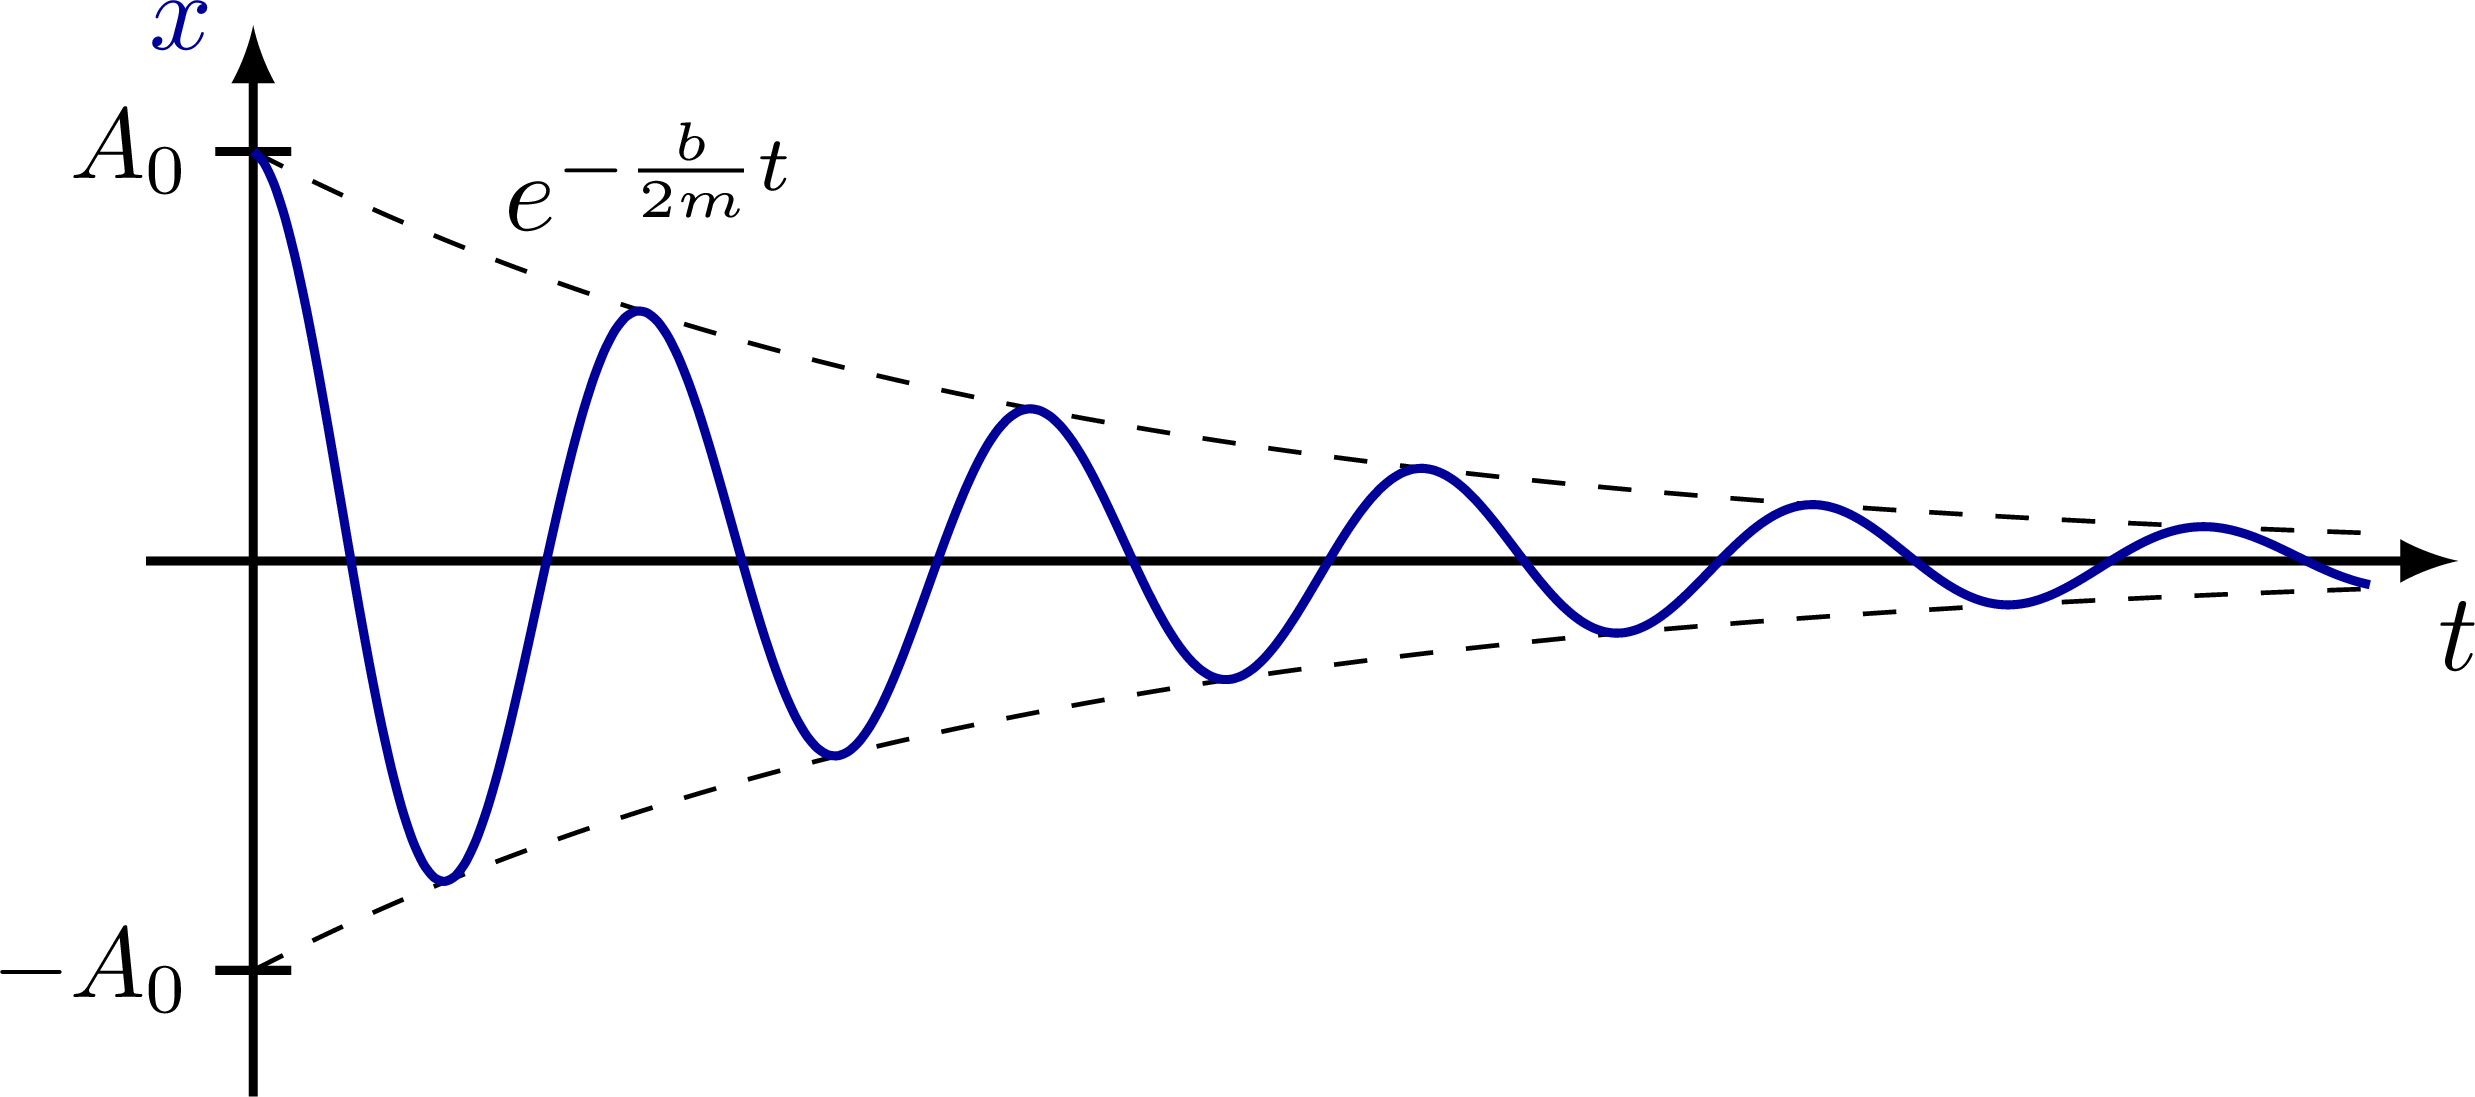
\includegraphics[width=0.9\linewidth]{images/resonances/dynamics_oscillator.png}
\caption{Visualization of the real part of a resonance with an exponential decay factor as an envelop (\cite{neutelings_harmonic_2021}).}
\label{dampedHarmonic} \vspace{3cm}
\end{marginfigure}

Signal $x$ is formed by a summation of different complex resonances with $d_k$ the initial complex amplitude of the oscillator and a rotating vector $e^{-i\omega_kt}$, dependent on the complex frequency $\omega_k$. It might seem illogical to see the notation of a continuous signal for discrete resonances (i.e., $x(t)$ instead of $x[n]$). We will leave the details behind this formulation beside, the important thing is to know that it is based on the Continuous Fourier Transform, and will only be discretized in the actual implementation.

Just to prevent confusion with the previous chapter: the definition of resonances describes a time-signal that is decomposed in damped or driven oscillators, just like Fourier series did for stationary signals. In resonances, a fourth dimension is added, containing the decay. In a 3D representation, the following visualization in Figure \ref{fig:resonace3D} of a resonance can give a more intuitive feeling for its appearance. The decay can be observed as the complex exponential function in Figure \ref{dampedHarmonic}.


\begin{figure}[ht]
    \centering
    \adjustbox{width=1\linewidth}{\resonance{}}
    \vspace{0.3cm}
    \caption{A visual representation of a resonance in 3D.}
    \label{fig:resonace3D}
\end{figure}

The complex frequency $\omega_k$ consists of a real and imaginary part, namely the frequency of the resonance $\phi_k$ and the rate of decay $\gamma_k$ as a complex part: $\omega_k = \phi_k +i \gamma_k$. A short mathematical interpretation illustrates the intuition behind this formulation: 

\begin{marginfigure}
\centering
\includesvg[width=0.9\linewidth]{images/resonances/resonanceComplex.svg}
\caption{A discrete resonance with the complex part visualized with dotted lines and the real part with the continuous line (\cite{homer_modelling_2023}).}
\label{resonanceComplex} 
\vspace{3cm}
\end{marginfigure}

\begin{equation}
\begin{split}
e^{-i\omega_kt} &= e^{-i(\phi_k + i\gamma_k)t}  \\
&= e^{-i\phi_k t + \gamma_k t} \\
&= e^{\gamma_k t}e^{-i \phi_k t} \\
&= e^{\gamma_k t} [\cos(\phi_k t)-i \sin(\phi_k t)] \\
&= e^{\gamma_k t} [\cos(\phi_k t)+i \sin(\phi_k t)]^*
\end{split}
\end{equation}

$\gamma_k$ describes the decay of the resonance, and the sine and cosine terms are a representation of the oscillatory behavior and denote the frequency.  Visually, one can think of it as decayed or augmented sine waves. 
Furthermore, $d_k$ can be rewritten as $|d_k|e^{i\psi_kt}$, with $\psi_k$ denoting the initial phase of the oscillator. The absolute value of the amplitude is the polar representation of $d_k$.
\begin{equation}
    x[t] = \sum^K_{k=1} |d_k|e^{i\psi_kt} e^{-i(\phi_k + i \gamma _k)t}  
    \; \; \; \; \; \; \; \; \; \; \; \; \; \;
    |d_k|, \psi_k, \phi_k, \gamma_k \in \mathbb{R}
\end{equation}



\section{Discrete Resonances in Frequency Domain}


The Fourier transform is a tool for performing spectral analysis of time-domain signals. It is defined with respect to frequency $\phi$. Here, the oscillatory signal is represented in the frequency domain:
\begin{equation}
    X(\phi) = \frac{i}{\sqrt{2 \pi}} \sum^K_{k=1} \frac{d_k}{\phi - \omega_k} = \frac{i}{\sqrt{2 \pi}} \sum^K_{k=1} \frac{|d_k| e^{i\psi_k}}{\phi - (\phi_k + i \gamma_k)}.
\end{equation}
The absolute value of the amplitude $d_k$ corresponds in the frequency domain to the size of the resonance peak. Frequency $\phi_k$ defines the location of the resonance peak, and decay $\gamma_k$ influences the width and polarity of the resonance peak in the frequency domain. Here, again, $\psi_k$ is the initial phase of the oscillator. In the frequency domain, it has an effect on altering the angle of the rotating vector, thus the cotangent of the angle: $\Re[f(\phi)]/\Im[f(\phi)]$. 

\begin{marginfigure}
\centering
\includesvg[width=0.9\linewidth]{images/resonances/resonanceFreqSpec.svg}
\caption{A discrete resonance in the frequency domain (\cite{homer_modelling_2023}).}
\label{resonanceFreqSpec} 
\end{marginfigure}

\section{The Fast Padé Transform (FPT)}

In section \ref{sec:FFT}, we briefly discussed the Fast Fourier Transform. The power for finding the coefficients hides in the specific selection and evaluation of complex numbers sitting evenly spaced on the unit circle, or, in other words, due to the restriction of having orthogonal bases in a Hilbert Space. 

However, when the complex numbers are not evenly spaced, and not even necessarily on the unit circle (which is the case for discrete resonances), it becomes a quite expensive operation to find those coefficients. Therefore, Steven Homer (personal communication, 2023) applied The Fast Padé Transform (\cite{belkic_signal_2019}) on resonances to estimate the spectral density function of a time series signal, which is a distribution of the power of a signal across different frequencies. The Fast Padé Transform itself is a numerical algorithm for approximating the power series expansion of a function in a given interval. It is a fast and efficient and can compute the coefficients of a Padé approximant, which is a rational function that interpolates the power series expansion of a function


\subsection{Preliminary Knowledge}
We will begin by refreshing key concepts from linear algebra. This primer will help establish a solid foundation for understanding the mathematical derivation of the Fast Padé Transform.

\begin{definition}[Generating function]
A generating function $G(x)$ encodes an infinite sequence of numbers by treating them as coefficients of a formal power series. 
\end{definition}
A simple example of a generating function is the encoding of even numbers with 

\begin{equation}
    G(x) = \frac{2x}{(1-x)^2}, 
\end{equation}

which will generate the sequence of even numbers $\{0, 2, 4, 6, 8, ...\}$. 

\begin{definition}[Constant-recursive sequence]
A constant-recursive sequence is an infinite sequence of numbers, where each number in the sequence is equal to a fixed linear combination of one or more of its immediate predecessors.
\end{definition}
This feature will be important in the further derivation, since the sequence is constant recursive, this will allow us to define analytic functions in a Hilbert space.

% \begin{definition}[Sequence versus series]
% A sequence orders the numbers in a certain order, when series refers to the summation of the terms.
% \end{definition}

% \begin{definition}[Closed-form expression]
% A mathematical expression that uses a finite number of standard operations.
% \end{definition}

% \begin{definition}[The fundamental theorem of algebra]
% The fundamental theorem of algebra states that every non-constant single-variable polynomial with complex coefficients has at least one complex root."
% \end{definition}


\subsection{Mathematical Derivation}
We will now discuss the rough structure of a mathematical derivation for the Fast Padé Transform originating from \textcite{belkic_signal_2019} and applied to the resonance spectrum by Steven Homer (personal communication, 2023).

Assume the ordinary generation function $G$ of the infinite constant-recursive sequence of numbers ($c_n$):
\begin{equation}
	G(c_n,z) = \sum_{n=0}^\infty c_n z^{n}.
\end{equation}
$z$ denotes a coordinate in polar representation (i.e., $e^{-iw_kt}$). 

By definition, a \textit{formal} power series does not have to converge, but since this generating function is defined to be an analytic function in a Hilbert Space, it means that it has a convergent power series expansion. The goal of the derivation is to come define a closed-form expression that can be evaluated and makes the definition valuable. Assuming that $c_n$ is constant-recursive sequence, the generative function can be rewritten as 

\begin{equation}
	G(c_n,z^{-1}) = \sum^\infty_{n=0} c_n z^{-n} =\frac{\sum\limits_{k=0}^{K-1}p^-_kz^{-K}}{1+\sum\limits_{k=1}^{K}q^-_kz^{-K}} \left( \frac{z^K}{z^K} \right)
\end{equation}

Which is a Padé approximate by definition. Note that, for the sake of math, a multiplicative inverse of the complex number $z$ was used. The modification to the negative angle does not change anything about the real value of the signal, since a real number is equal to a complex number (no matter positive or negative) with its imaginary part equal to zero. The negative annotation at the coefficients was introduced to denote that they are a coordinate in the negative domain. After the derivation, it returns to the positive domain. The derived generic function can be rewritten as




\begin{equation}
	\sum^\infty_{n=0} c_n z^{-n} = \frac{\sum\limits^K_{k=1} p_k z^k}{1+\sum\limits^K_{k=1}q_kz^k}
 %z \frac{p_{k-1}^+(z)}{q_k^+(z)}
\end{equation}

This equation is solvable by deriving this equation with respect to the variable $z$. By introducing the initial complex amplitude $d_k$, the equality can be rewritten as

\begin{equation}
    \sum^K_{k=1} \frac{d_k}{1-(\frac{z_k}{z})}
\end{equation}


For a full derivation, please read \textcite{belkic_signal_2019}, page 65-77). This form looks exactly as a geometric series $\sum^\infty_{n=0}ar^n=\frac{a}{1-r}$, with $|r| < 1$ and thus if the following inequality holds: $|\frac{z_k}{z}|<1$, the equality can be written as

\begin{equation}
 \sum^K_{k=1} d_k \sum^\infty_{n=0}(\frac{z_k}{z})^n.
\end{equation}
Therefore,
\begin{equation}
    c_n = \sum^K_{n=1} d_k z_k^n.
\end{equation}

Notice that $z_k$ represents the complex plane. The derived summation represents a function in $n$. If the signal is a simple cosine, then it moves around the unit circle when n increases. In the case that the frequency is complex, and the decay is non-zero, the coordinates will fall inside or outside the unit circle. In other words, $c_n$ can be expressed as a sum of oscillators. Solving this equation for $d_k$ and $z_k$ is exactly what the FPT does in a certain interval, i.e., rectangular window, defined as following:

\begin{equation}
    \sum^\infty_{n=0} c_n z^{-n} - \sum^\infty_{n=N} c_n z^{-n}
\end{equation}
Solving the equation by substituting it with the derivation we had before, gives us
\begin{equation}
    \sum^{N-1}_{n=0} c_n z^{-n} = \frac{\sum\limits_{k=1}^K p_k z^{k}+\sum\limits_{k=1}^K r_k z^{k-N}}{1+\sum\limits_{k=1}^K q_kz^k}
\end{equation}
For a window function where $p$ and $r$ represents the coefficients at the left and right side of the window. which is exactly the FPT (can also be seen as a convolution). Essentially, this derivation allows us to find the $c_n$'s and $z$, and therefore the oscillators. And since K = N/2, there is a unique solution.

\begin{marginfigure}
\centering
\includesvg[width=0.9\linewidth]{images/resonances/resonance_circle.svg}
\caption{A pole-zero diagram consisting of distinct points that are not uniformly distributed due to the non-orthogonal bases and are no longer located on a unit circle due to the complex frequency $\omega_k$.}
\label{resonanceCircle} \vspace{3cm}
\end{marginfigure}

\subsubsection{Non-Orthogonal Bases in a Hilbert Space}

Although the usage of orthogonal bases ensures efficient computation and a simple representation, using a collection of non-orthogonal basis functions can be advantageous in some cases, such as in the Hilbert Space of Resonances. The non-orthogonal bases allow us to have non-evenly spaced frequencies $\gamma_k$, which is a sequence of numbers. By gaining more freedom with the placement of the frequencies in this space, the frequencies of a signal can be found more precise without limiting itself to a sample rate, as illustrated in Figure \ref{resonanceCircle}, and a bigger space in the complex plane can be explored.

Consider now the normalized sequence of signals




\begin{equation}
    \phi_k(t) = e^{i \omega_k t}  \; \; \; \; \; \; \; \; , k \in \mathbf{Z}.
\end{equation}

Here, $\omega_k$ is a sequence of numbers and if  $\omega_k$ = k, we obtain the classical Fourier series basis, with $\phi_k$ an orthogonal basis. 
However, if $\omega_k$ is not an integer multiple, the signals are not orthogonal (\cite{romberg_ece_2016}). Since $\omega_k$ is a complex function in our application of resonances (a complex frequency that makes the sinusoidal decay), we do not have evenly spaced points anymore in the discretization of the formula, as is shown in Figure \ref{resonanceCircle}.
The reason why a signal can equivalently be decomposed into resonances, as Fourier analysis does with sines and cosines, is because
\begin{marginfigure}
\centering
\vspace*{-7cm}
\includesvg[pretex=\fontsize{4pt}{6pt}, width=0.9\linewidth]{images/fftvsfpt/stft_a4_top.svg}
\label{topview_stft} 
\end{marginfigure}
\begin{marginfigure}
\vspace*{-1.6cm}
\centering
\includesvg[pretex=\fontsize{8pt}{10pt}, width=0.9\linewidth]{images/fftvsfpt/stft_a4.svg}
\caption{A filtered Fourier spectrogram showing the fundamental A4 and its overtones performed by a flute.} 
\label{fourierSpectrogram} 
\end{marginfigure}
\begin{marginfigure}
\centering
\vspace*{1.2cm}
\includesvg[pretex=\fontsize{4pt}{6pt}, width=0.9\linewidth]{images/fftvsfpt/fpt_a4_top.svg}
\label{topview_fpt} 
\end{marginfigure}
\begin{marginfigure}
\centering
\includesvg[pretex=\fontsize{8pt}{10pt}, width=0.9\linewidth]{images/fftvsfpt/fpt_a4.svg}
\caption{A filtered resonance spectrogram representing the same fundamental A4 and its overtones performed by a flute. Note the high precision of this method.}
\label{resonanceSpectrogram} 
\end{marginfigure}
\begin{equation}
    e^{\gamma t} cos(\phi_k t) = \frac{1}{2}( e^{i (\phi_k + i \gamma_k) t} +  e^{-i (\phi_k - i \gamma_k) t}).
\end{equation}
Summarized, $\braket{f|g} = 0$ is not required to be true from an algebraic point of view and the complex frequency with a decaying factor uses non-orthogonal basis.




\section{Towards higher Precision with Non-Orthogonal Bases in a Hilbert Space}
\label{sec:nonorthogonalBases}

Due to the non-orthogonal property of the Fast Padé Transform, the size of each frequency bin in a time slice is varying with respect to the parameters of a resonance. This has enormous advantages in terms of precision when performing spectral analysis. Figures \ref{fourierSpectrogram} and \ref{resonanceSpectrogram} provide a visual demonstration of the fundamental difference between the widely used Short Time Fourier transform and the Fast Padé Transform with a synthetic audio recording of a flute performing the musical note A4. The visualized signals were filtered on power and frequency for the purpose of simple visualization of the main difference between the two methods. The frequency was set in a range between 0 and 2000 since the fundamental frequency and its observable harmonics generally lay between this range (\cite{huang_resonance-based_2017}). Resonances with a relatively small power were also removed from both plots.
In Figure \ref{fourierSpectrogram}, the resolution of the time and frequency domains are fixed and bound with the STFT, and due to that, the signal is estimated with a division over several nearest frequency bins, bounded by Heisenberg's uncertainty principle (\cite{folland_uncertainty_1997}). However, due to the non-orthogonal requirements of the basis, the size of frequency bins may vary and a more precise estimation of the frequency components can be achieved.


 \section{Extracting Attributes from the Discrete Resonance Spectrum}
 \subsection{Dynamic Resonances}
 The dynamic resonance is a non-explicitly documented technique (Homer, personal communication, 2023), wherein different distance metrics were used to combine two resonances in consecutive slices with each other. The six distance measures were defined as following: frequency distance, harmonic mean of the $d_k$ and $w_k$ coefficients, residue of the product of the resonances, residue of the product of the resonances weighted by power, residue of the product of the resonances multiplied by the spectra transference function and residue of the product of the resonances multiplied by the spectra transference function weighted by power.

A dynamic resonance is a relation of the distance metric $d$ defined as following:



\begin{definition}[dynamic resonance]
Let $S_x$ and $S_{x+1}$ be non-empty consecutive slices in a spectrogram $S$ with distinct resonances, and let $d(i, j)$ be a distance function defined for all pairs $(i, j)$ representing those resonances, such that $i \in S_x$ and $j \in S_{x+1}$. We define the relation $R$ as follows: 

\begin{equation}
    \forall i \in S_x, \exists j \in S_{x+1}: d(i,j) \leq d(i,k) \; \; \;  \; \; \forall k \in S_{x+1} \smallsetminus \{j\}.
\end{equation}

\end{definition}

\begin{marginfigure}
\centering
\includesvg[pretex=\fontsize{8pt}{10pt}, width=0.8\linewidth]{images/cluster/measurement.svg}
\vspace{0.1cm}
\caption{Two consecutive slices $S_x$ and $s_{x+1}$ and the relation between two resonances measured with a distance function $d$.}
\label{distanceMeasurement} 
\end{marginfigure}

 \begin{marginfigure}
    \centering
    \vspace{2cm}
    \includesvg[ width=1\linewidth]{images/cluster/dynamicResonances.svg}
    \caption{Dynamic Resonance spectrum.}
    \label{fig:DynamicResonance}
\end{marginfigure}

Due to the slow computational speed of Python and excessive usage of loops, his approach worked significantly slower than our density based approach. However, the insight of using other distance measurements than the Euclidean for the definition of distance inspired us to measure similarity between resonances with the following definition:
 

\begin{equation}
    \cos (d_{jk}) = \frac{\Re \left[\frac{d_jd_k}{w_j-w_k}\right]}{\frac{|d_j|^2}{\gamma_j}\frac{|d_k|^2}{\gamma_k}}
\end{equation}

After implementing and evaluating this approach, the distance measurement based on similarity of resonances did not contribute to a better clustering. However, it can serve as an inspiration for using other distance measurements in future work to extract more features from the data.


\section{Summary}
We started this chapter with the definition of the discrete resonances in the time and frequency domain and summarized the proof of the Fast Padé Transform, which is a discrete convolution of the coefficients $c_n$ with the coefficients $q_k$, yielding the coefficients $p_k$ and $r_k$ and zeros. We showed that the main difference with Discrete Fourier Transform is the use of a non-orthogonal basis in a Hilbert Space. We introduced \textit{dynamic resonances} as a novel method for grouping resonances. However, it requires high computational power and therefore, we will introduce a cognitive-based method for cluster analysis for the extraction of musical structures from the discrete resonance spectrum.



 
    \chapter{Cluster Analysis of Resonances}
\label{chap:cluster}

\begin{marginfigure}
\vspace{6cm}
\includesvg[ width=1\linewidth]{images/cluster/kmeans.svg}
\caption{The resonances in this figure is a representation of the resonances with the strongest power, extracted from the sound of a flute playing the note A4. They are clustered by the K-means algorithm ($K=4$) and each cluster is represented with a different color.}
\label{kmean} 
\end{marginfigure}

\begin{marginfigure}
\includesvg[ width=1\linewidth]{images/cluster/dbscanFlute.svg}
\caption{Resonances clustered by the DBSCAN algorithm ($\epsilon=0.4$, $minPts = 4$) are represented with different colors. The labeling mimics how a human would draw circles around resonance groups to extract specific features, which exactly aligns with our desired outcome.}
\label{dbscanFlute} 
\end{marginfigure}

Clustering is an unsupervised machine learning technique that involves grouping similar data points based on a specific parameter, such as density or similarity. There are various models known in the literature, with K-means being a conventional one that generates a fixed number of clusters associated with a central point. The Markov Cluster Algorithm, introduced by Stijn \textcite{van_dongen_graph_2008}, is more appropriate for graphs/networks. Hierarchical clustering on the other hand is often used for the analysis of social network data and biological data analysis (\cite{hexmoor_diffusion_nodate, yeturu_chapter_2020}). An important drawback of both K-means and hierarchical clustering for our application is that they do not automatically determine the number of clusters. Density-based algorithms, however, such as Mean-Shift, DBSCAN, and HDBSCAN, are more appropriate for this particular problem: resonances require a density-based approach (sudden changes of dense regions imply new musical objects), and they are also capable of automatically determining the amount of clusters based on the input data.
The previews provided in Figure \ref{kmean} and \ref{dbscanFlute} highlights the benefits of using density-based algorithms for resonance data. 


\section{Density-based Cluster Algorithms}

First, let us provide a concise overview of the three density-based cluster algorithms mentioned above. The iterative Mean-Shift algorithm moves each data point towards the mean of its respective region to form clusters. This is a centroid-based algorithm and works best for blob-shaped data. DBSCAN is capable of identifying outliers as noise, unlike the Mean-Shift method, and performs effectively on densely populated data with irregular shapes. HDBSCAN is a variation of DBSCAN introduced by \textcite{campello_density-based_2013}. In this algorithm, DBSCAN's principle of border points (see further) is abandoned, and only core points are considered as part of the cluster. Even though this method may be beneficial for handling noisy data, DBSCAN is nonetheless deemed to be the most appropriate clustering model for this problem, as it is better to implement custom filtering methods for noise reduction before performing clustering.

\section{DBSCAN clustering algorithm}
\begin{marginfigure}
\vspace{0.5cm}
\centering
\includesvg[ width=0.5\linewidth]{images/cluster/dbscan1.svg}
\vspace{0.1cm}
\caption{\textbf{Step 1} | Select a point $p$ and assume minPts = 3 and $\epsilon$ = 0.1. If at least 3 points are inside radius, mark $p$ as a core point.}
\label{dbscan1} 
\end{marginfigure}

\begin{marginfigure}
\centering
\includesvg[ width=0.5\linewidth]{images/cluster/dbscan2.svg}
\vspace{0.1cm}
\caption{\textbf{Step 2} | Iterate over each point and mark all core points, classify left-overs as non-core points.}
\label{dbscan2} 
\end{marginfigure}

\begin{marginfigure}
\centering
\includesvg[ width=0.5\linewidth]{images/cluster/dbscan3.svg}
\vspace{0.1cm}
\caption{\textbf{Step 3} | Pick a random core point, assign it to the first cluster together with all core points in the radius.}
\label{dbscan3} 
\end{marginfigure}

\begin{marginfigure}
\centering
\includesvg[ width=0.5\linewidth]{images/cluster/dbscan4.svg}
\vspace{0.1cm}
\caption{\textbf{Step 4} | Repeat for the neighbouring core points.}
\label{dbscan4} 
\end{marginfigure}

\begin{marginfigure}
\centering
\includesvg[ width=0.5\linewidth]{images/cluster/dbscan5.svg}
\vspace{0.1cm}
\caption{\textbf{Step 5} | Once all the core points have been included in the initial cluster, the border points, which are non-core points within the radius of the core points, are added to the same cluster as well. Note that these border points are not extended iteratively.}
\label{dbscan5} 
\end{marginfigure}

\begin{marginfigure}
\centering
\includesvg[ width=0.5\linewidth]{images/cluster/dbscan6.svg}
\vspace{0.1cm}
\caption{\textbf{Step 6} | Repeat this process to find all clusters. Points that do not belong to any cluster are called noise points and are marked with red.}
\label{dbscan6} 
\end{marginfigure}
Density-based Spatial Clustering of Applications (DBSCAN: \cite{ester_density-based_1996}) is a data based clustering algorithm. The algorithm attempts to imitate the human ability to recognize groups of points with an arbitrary shape that are closely located to each other, and singles out isolated points as noise.
Figures \ref{dbscan1}-\ref{dbscan6} visualize the DBSCAN algorithm step by step.
The model estimates the minimum density level using a method that relies on a threshold value, minPts, for the number of neighbors within a radius $\epsilon$. The algorithm begins by marking all core points in the dataset. A point $p$ is classified as \textbf{core point} if there are at least minPts points (including $p$) within the radius $\epsilon$. In the next step, a random core point $i$ is selected from which all transitively included (i.e.,density-reachable) core points are identified to form a cluster. Then, all \textbf{border points}, which are non-core points in the radius of a core point, are added to the cluster of a core point. Notice that a border point that is in the radius of two core points of different clusters will just be classified in the first cluster that is processed. Any points that are not density reachable from any core points are classified as noise and do not belong to any cluster. To ensure that all points in the same cluster are included, the minimum number of points (minPts) should be set to a relatively low value (\cite{ester_density-based_1996, schubert_dbscan_2017}).


\subsection{Complexity and Data structure}
Multiple implementations of the DBSCAN algorithm exist. A more optimized implementation utilizes a FIFO queue to keep track of the points which are already labelled and a $R^*$-tree, Kd-tree, or cover tree for performing a continuous search for density points within a tree-like structure (\cite{schubert_dbscan_2017}). The average time complexity is $O(n\log(n))$, since the neighboring queries are executed in logarithmic time, and labeling core and non-core points takes $O(n)$. Worst case, with degenerate data or naive implementations (e.g., not using the index structure), the time complexity becomes $O(n^2)$. We use an adjacency list-based implementation, which is better in terms of running time and memory usage compared to the matrix-based implementation.


\subsection{DMBSDSCAN}
A drawback of  DBSCAN is that it performs less well at data with a wide variation in density. DMDBSCAN attempts to solve this problem by introducing a dynamic $\epsilon$ estimation, suitable for each density level in the dataset (\cite{elbatta_dynamic_2013}). The algorithm is suggested for future work in case that the static $\epsilon$-estimation would not be sufficient. The required accuracy can currently be pre-defined and adjusted by the user.


\section{Summary}
We delved into a density-based clustering approach, in which labeling mimics how a human would draw circles around resonance groups when plotting it in a certain dimension. The next section will introduce a hierarchy wherein we will be able to represent the obtained clusters and attribute them.
    \setlength{\headheight}{23.84448pt}
\addtolength{\topmargin}{-10.84448pt}

\chapter{Type-Based Knowledge Representation}
\label{chap:knowledge}

\textcite{shi_cognitive_2019} introduced the evolution of the human brain, denoting that the appreciation of music by the brain cortex coincided with the development of human abstract thinking.
Knowledge is the possession of the ability to locate information, and therefore, we will introduce Harley's type-based framework for the abstract representation of musical knowledge (\cite{harley_abstract_2020}).
His framework uses a constituent structure (i.e., a multi-hierarchical information model) that is able to represent the complex hierarchies of musical spaces. The framework has a main, extendable module named CHAKRA, which gives the user the freedom to create structures in terms of constituents, attributes and hierarchies. A submodule of CHAKRA, named CHARM (\cite{wiggins_representing_1989}), is a particular representation system for the creation of music-specific multidimensional hierarchies. First, we will emphasize the difference between knowledge and data, followed by highlighting the importance of the type-based aspect of the CHAKRA framework, by introducing three perspectives on computation: Type theory, Category Theory and Typed logic. Afterward, the components of the CHARM system will be briefly defined, serving to understand our own software architecture, introduced in part III.


\section{The Three Perspectives on Computation}

\begin{marginfigure}
    \centering
    \includesvg[pretex=\fontsize{8pt}{10pt}, width=1\linewidth]{images/knowledge/trinity.svg}
    \vspace{0.5cm}
    \caption{Computational Trinity: a tripartite correspondence between Logic, Type Theory, and Category Theory.}
    \label{typeTheory}
\end{marginfigure}

The Three Perspectives on Computation, also called \textit{The Computational Trinity}, is the central organizing principle of a theory of computation that unifies Logic, Type Theory, and Category Theory (\cite{eades_type_2012, goguen_categorical_1991}). The three fields look different but are nevertheless equivalently treatable. One may think of it more intuitively as the unification of a subfield of logic, programming, and mathematics, wherein every proof can be written as a program, every program corresponds to a mapping, and every mapping to a proof (\cite{harper_holy_2011}). 

\subsection{Type Theory}
At the early 20th century, Bertrand Russell introduced type theory to cope with a paradox in naive set theory, which was expressed as follows:
\begin{equation}
    H = \{ x | x \notin x\} \Rightarrow H \in H \Leftrightarrow H \notin H.
\end{equation}

The paradox arises when one considers whether $H$ contains itself or not. If $H$ contains itself, then by definition it is a set that does not contain itself, which is a contradiction. On the other hand, if $H$ does not contain itself, then by definition it is a set that should contain itself, which is also a contradiction. This problem arises when impredicative universal quantification is allowed, which means that the definition of the object involves quantifying over all objects, including the object being defined itself. Russel's type theory resolved this problem by defining objects as part of a specific group. Consider a type n, then we can redefine $H$ as
\begin{equation}
    H^n = \{ x^{n-1} | x^{n-1} \notin x^{n-1}\} \Rightarrow H^n \in H^n \Leftrightarrow H^n \notin H^n.
\end{equation}
In this case, the paradox is false since the sets are defined by the types, and type $n-1$ excludes type $n$ (\cite{eades_type_2012}).

\begin{marginfigure}
\centering
\includesvg[width=0.8\linewidth]{images/knowledge/category.svg}
\vspace{0.5cm}
\caption{Category $C$ with a set of objects $\{X, Y, Z, W\}$, morphisms $\{f, g, h\}$ and composition of morphisms $\{f \circ g \}$. Each object also has an identity morphism: an arrow points to the object itself. }
\label{categoryGraph} 
\end{marginfigure}

Type theory became the formal presentation that models objects and relations, such as a variable, function or substitution, with types. For example, variable 10 has the type of natural numbers ($\mathbb{N}$), which is in the built-in notation written as $10: \textrm{nat}$. From this term, other typed terms can be constructed. As illustrated in (\cite{hoang_type_2014}), terms of the type $\mathbb{N}$ can be constructed just by defining the variable as we defined before, or as a successor function $succ(n) : \mathbb{N}$:

\begin{figure}[h]
\centering
\includesvg[width=1\linewidth]{images/knowledge/typeSuccessor.svg}
\label{category} 
\end{figure}


\subsection{Category Theory}
Tom Leinster described category theory as a bird's eye view of mathematics. From high in the sky, details become invisible, but we can spot patterns that were impossible to detect from ground level (\cite{leinster_basic_2016}). Formally, category theory is the study of mathematical structures using abstractions of functions called morphisms, as well as a mathematical workspace and theory (\cite{barr_category_2012, eades_type_2012}). It provides the concepts to meaningfully compare and combine unrelated systems by understanding their patterns (\cite{harley_abstract_2020}). 
A category $C$ is an abstract object consisting of a set of objects, morphisms and compositions of morphisms. The objects and relations can visually be represented as directed graphs, as illustrated in figure \ref{categoryGraph}.

\begin{marginfigure}
    \centering
    \vspace{2cm}
    \includesvg[width=1\linewidth]{images/knowledge/functor.svg}
    \vspace{0.2cm}
    \caption{A functor represented as a directed edge from category $C$ to category $D$.}
    \label{functor}
\end{marginfigure}

 Categories are connected through structure-preserving maps named functors. They can be considered as morphisms in a category of subcategories.
 This theoretical framework of formalization is especially useful for combining different levels of abstraction (e.g. the unification of CHARM with other modules as will be explained further), and for formal descriptions of systems.

\subsection{Typed logic}
\label{sec:cic}
The perspective on type theory, from a logical aspect, is the definition of certain rules that must hold. An example of a formal language using these inference rules for programming purposes, is Calculus of Inductive Constructions (Cic). An example of a typing rule in Cic is defined as following: 

\begin{equation}
\frac{E[\Gamma] \vdash T: s \quad s \in \mathcal{S} \quad x \notin \Gamma}{\mathcal{W} F(E)[\Gamma::(x: T)]}
\end{equation}



Where a term $t$ is correctly typed in a global environment $E$ if and only if there exists a local context $\Gamma$ and a term $T$ such that the judgement  $E[\Gamma] \vdash t:T$ can be derived from the following rules, as literally mentioned by \textcite{inria_calculus_2018}. However, the interpretation of this rule is not important in context of the thesis and only serves as an illustration.

 
\section{The CHAKRA System}

Type theory is a strong and important foundation for the implementation of the \textit{Common Hierarchical Abstract Knowledge Representation for Anything} (CHAKRA) framework, since it allows the integration of heterogeneous data and avoids the paradox of naive set theory. CHAKRA was originally defined in Coq\footnote{https://nick-harley.github.io/chakra-coq/chakra.html}, a library with Calculus of Inductive Constructions as underlying formal language (a mapping from logic to programming). Afterward, an implementation of the CHAKRA-framework was written in Julia \footnote{https://github.com/nick-harley/Chakra}.



\subsection{The CHARM System}
The \textit{Common Hierarchical Abstract Representation of Music} (CHARM) intends to provide a logical specification of an abstract representation of music
(\cite{pearce_construction_2005, wiggins_representing_1989}), regardless of the particular style, data source or application (\cite{smaill_hierarchical_1993}). It inherits the abstract structural components Constituent, Id and Hierarchy from CHAKRA and applies it in the musical domain (\cite{harley_charm_2022}). 


\subsubsection{Musical Objects with Attributes in a Space}
Musical objects are seen as statements about the world in the musical space. These atomic entities automatically add semantics to data wherefore they can be considered as \textbf{knowledge}, rather than data. Note that data can be seen as the simplest form of raw values. Knowledge, in contrast, is a statement about something in the world space that could be true or false.

\begin{marginfigure}
\centering
\includesvg[pretex=\fontsize{7pt}{9pt},width=1\linewidth]{images/knowledge/constituent.svg}
\caption{A simplification of a constituent $c_1 \in C$ defined in the musical space $M$.}
\label{constituent} 
\end{marginfigure}


We call every existent musical object a \textit{Constituent} and use them in a hierarchical structure. Musical objects contain attributes such as $frequency$, $amplitude$ and $onset$ which can be defined in an (abstract) musical space. Often the attribute name and the name of the space is the same (for example, the attribute pitch and musical space pitch). However, sometimes they do not overlap (for example, the attributes \textit{onset} and \textit{off-set} both have the musical space of time, but it is important that their attributes names are different) (\cite{harley_abstract_2020}). In Figure \ref{constituent}, an example of a musical object (i.e., constituent) is given. The constituent is formed from a joint pair of resonance $r_1$ and $-r_1$, and has 10 attributes. The attributes of musical objects are equivalent to the features of a dataset.




\subsubsection{Definitions}

The first concept defined in CHARM, is the Constituent $C$, a high-level grouping of musical objects defined in (multiple) musical spaces $M$ (\cite{wiggins_representing_1989}). Musical objects are atomic entities of the human conceptualizations of music, such as resonances, slices in time of an audio signal or onsets of notes. The set of locations in musical space $M = (M_a)_{a \in A}$ is a family of sets indexed by attributes $A$ and $M_a$ is the subspace or dimension indicated by the perspective $a$ \parencite[p. 111]{harley_abstract_2020}. For example, a constituent representing a resonance, contains the attributes frequency, onset, decay and amplitude. 
\begin{theorem}[Attribute]
\label{Attribute}
The set of Attribute names $A$ is a collection of keys for key-value pairs, where key $a \in A$.
\end{theorem}

Constituents are used to construct hierarchical structures. They are connected in a directed acyclic graph and its relation is called a Hierarchy $H$. Note that a single constituent can be defined in multiple hierarchical structures.


\begin{definition}[Constituent]
\label{def:constituent}
 A musical object (i.e., a constituent) is composed of a tuple <i, P(i), R(i)> where identifier = $i$, particles = $P(i)$ and attributes =$R(i)$ \parencite[p. 112]{harley_abstract_2020}.
 \end{definition}
We explicitly use the notation R(i) here instead of A because A is the set of names and R a set of relations between constituents and values. Thus, $(a,v) \in R_i$ means that the value of an attribute should be taken.
 
\begin{marginfigure}
\centering
\includesvg[pretex=\fontsize{10pt}{12pt}, width=0.7\linewidth]{images/knowledge/constituent_tuple.svg}
\vspace{0.2cm}
\caption{A constituent $C$ consisting of the identifier, particles and attributes.}.
\label{hierarchy} 
\end{marginfigure}


\begin{definition}[Hierarchy]
\label{Hierarchy}
$H \subset C \times C$ is a binary relation $C$, such that $(C, H)$ forms a (simple) directed acyclic graph (DAG).  The graph $(C,H)$ captures the hierarchical structure of the domain, where $(c, c') \in H$ indicates that $c'$ is part of $c$ \parencite[p. 111]{harley_abstract_2020}.
\end{definition}

 
\section{Summary}
We introduced the CHAKRA system as a model for the human-like ability to locate and use information. The theoretical underpinnings of this framework were explored from three different perspectives, providing a better understanding of its principles. Finally, we defined the constituent elements of CHAKRA in context of music, setting the foundation for the actual implementation in the following part.



    %%%%%%%%%%%%% PART 3 %%%%%%%%%%%%%%%%%
    
    \begin{adjustwidth}{2cm}{-6cm}
    \epigraphhead[550]{In this last part, we will demonstrate our own contribution, holding the connection between the \textit{already} developed model of perception with our own model of cognition and knowledge representation. We will start with the section that introduces our knowledge representation, since it gives an overall view of obtained clusters of constituents. The hierarchies can generally be categorized in four musical levels: frame-level, note-level, stream-level and notation-level (\cite{benetos_automatic_2019}). We demonstrate the possibilities of the developed software for a note-level description of music and touch the frame-level description with a first proposition. }\thispagestyle{empty}
    \part{Software Architecture}
    \end{adjustwidth}

    \chapter{Knowledge Representation Applied to Audio Files}
\label{chap:architecture}

\section{Specification of the CHAKRA abstraction}
We created a constituent structure (i.e., a multi-hierarchical information model) to model a theoretical estimation of the underlying structure of perception discussed in \ref{subsec:structualism} Structuralism. This constituent structure was an expansion of Harley's type-based framework for the abstract representation of anything. Learning and expanding knowledge about musical data was achieved through density-based clustering techniques. The acquired knowledge creates new dimensions in the hierarchical structure and gives more structural insights about musical structures in audio fragments. We will start with a discussion of the components of the music-specific CHAKRA implementation on resonances. Afterward, we briefly explain several engineering considerations during the development of this software. 


The central concept of the CHAKRA system is that it establishes the fundamental abstract types known as a \textit{Constituent, Identifier} and \textit{Hierarchy}. The user of this framework is then responsible for creating a customized implementation for these abstract types, inheriting their underlying structures.


\subsection{Constituent}
Every musical object in the hierarchical structure is called a \textit{Constituent}. New constituents are formed from finite sets of other constituents and are composed of an identifier $i$, particles $P(i)$ and attributes $R(i)$, as has been defined in \ref{def:constituent}. The value of an identifier is unique in a single set of identifiers. We call particles the children of a constituent (i.e., node) and the attributes are specific features of a constituent (e.g., onset, pitch, duration).


\begin{marginfigure}
\vspace{3cm}
\centering
\includesvg[pretex=\small, width=1\linewidth]{images/knowledge/constituent_flat.svg}
\vspace{0.1cm}
\caption{Visualization of a constituent containing a joint pair of resonances and its musical spaces.}
\label{constituentRes} 
\vspace{1cm}
\end{marginfigure}


\subsubsection{Constituents of a DRS}
The smallest musical objects in our particular hierarchy are resonances, they lay at the lowest layer of the hierarchy. 
We define each resonance as a constituent, containing 10 attributes, as illustrated in Figure \ref{constituentRes}. 

Each resonance has a conjugate pair with similar attributes; although the conjugate has the opposite sign of the frequency. For sake of completeness, the imaginary part of the signal is kept and the resonance and its conjugate are combined in a new \textit{pair}-constituent. From those pairs, slices in time are taken. A slice is defined as a small period of time containing a subset of the resonances (Figure \ref{slice}). These slices are, in their turn, grouped by a DRS-constituent. This constituent represents all the resonances in the time-domain of a Discrete Resonance spectrum.

\begin{marginfigure}
\centering
\includesvg[pretex=\fontsize{8pt}{10pt}, width=1\linewidth]{images/architecture/time-slice.svg}
\vspace{0.1cm}
\caption{A rough illustration of a slice in the time-domain representation of a signal. All musical objects falling inside a time-slice $t_n$ are grouped together by a slice constituent.}
\label{slice} \vspace{2cm}
\end{marginfigure}

\begin{figure}[h]
\centering
\includesvg[pretex=\fontsize{8pt}{10pt}, width=1\linewidth]{images/architecture/DRS.svg}
\vspace{0.1cm}
\caption{Two-dimensional hierarchical structure of the DRS hierarchy, consisting of four levels of constituents, denoted with circles.}
\label{drs} 
\end{figure}


\subsection{Identifier}

\begin{marginfigure}
\centering
\includesvg[pretex=\fontsize{12pt}{14pt}, width=0.5\linewidth]{images/architecture/id.svg}
\vspace{0.3cm}
\caption{A constituent $c_1$ and its corresponding ID $i_1$.}
\label{id} \vspace{2cm}
\end{marginfigure}

\begin{marginfigure}
\centering
\vspace{1cm}
\includesvg[pretex=\fontsize{8pt}{10pt}, width=0.9\linewidth]{images/architecture/set_constituent.svg}
\vspace{0.3cm}
\caption{The different sets of constituents and their corresponding IDs allows them to have similar names as long as they are defined within a different set.}
\label{setConstituent} 
\end{marginfigure}



The relation between Constituents and Identifiers is bijective in the multidimensional hierarchical structure. Their value can be repetitive through different sets, but will always contain a unique value in a single set of identifiers (e.g. ResIDs). The identifiers are important assets for finding components of Constituents. By returning the identifiers of the underneath level instead of the knowledge, improvements over speed and memory are achieved. Figure \ref{setConstituent} emphasizes the usage of sets for the definition of different IDs.


\subsection{Hierarchy}
A Hierarchy $H$ is a direct acyclic graph of constituents and is defined as the abstract type \textit{Hierarchy}. Subtypes of \textit{Hierarchy} directly correspond to specific implementations of this abstract type.  We will now explore four implementations of the hierarchies currently being developed, which can be further expanded by incorporating additional machine learning techniques.


\subsubsection{Definition of Several hierarchies}



The \textbf{DRS hierarchy} originates from the idea of a Discrete Resonance Spectrum. It groups resonances (both negative and positive) based on information from the time domain. Note the difference between the DRS constituent and the DRS Hierarchy. Although they have the same name, they do not hold the same semantic value.
Since half of the resonances are a subset of the negative part, they are often not needed for the analysis of real audio signals. Therefore, we defined the \textbf{NEG hierarchy} to group the resonances with a negative frequency together. This connection can make filtering easier if the imaginary part of the signal is not required. The \textbf{NOTE Hierarchy} was created for the extraction of musical notes from spectral data. The constituent representing a musical note is defined attributed with \textit{onset, duration} and \textit{pitch} and can formally be defined as following:
\begin{marginfigure}
\centering
\includesvg[width=1\linewidth]{images/architecture/hierarchyDynR_labeled.svg}
\caption{Real-valued representation of the DRS and HARM hierarchy for an audio fragment of a flute playing A4. The blue-like points are part of the DRS structure, including the resonances, pair, slice and DRS constituents. The orange points represent the constituents of the HARM hierarchy (the graph was generated with Gephi).}
\label{DRS_hierarchy_gephi}
\end{marginfigure}

\begin{equation}
    \text{NOTE\_Dataset}:\text{CSPEC} := \forall_{\text{Parts}}(\text{Note})
\end{equation}

Where CSPEC is the \textit{type} of constituent specifications defined in Calculus of Inductive
Constructions (see Chapter \ref{sec:cic}). Finally, the \textbf{HARM Hierarchy} contains constituents of overtones corresponding to a specific fundamental tone. A conceptual representation of the four hierarchies is represented in Figure \ref{DRS_hierarchy_prac} and a real-valued representation of the DRS and HARM hierarchies has been plotted in Figure \ref{DRS_hierarchy_gephi}.

\begin{figure}[h]
\centering
\vspace{0.5cm}
\includesvg[width=1\linewidth]{images/architecture/DRS_hierarchy_prac.svg}
\vspace{0.1cm}
\caption{A practical visualization of the state-of-the-art hierarchies in our software. Each hierarchy is visualized in its own color, containing Constituents represented as nodes.}
\label{DRS_hierarchy_prac} 
\end{figure}

\subsection{Operations}
The two most important operations in the hierarchical structures are \textit{parts} and \textit{find}. Parts gives all the particles of a selected constituent. The find operation returns all the attributes of a constituent or collection of constituents.

\section{Engineering Considerations}
We chose to use Julia for knowledge representation modeling and generating new constituents in the hierarchies. This decision was primarily influenced by two factors: firstly, the existing implementation of CHAKRA in Julia, and secondly, the superior speed performance of this uniquely typed language compared to other high-level languages like Python. Julia has many features, wherefrom multiple dispatch and duck typing are far away the most interesting to mention for our application. Multiple dispatch allows multiple functions with the same name, which is fast and was consequently exploited in the implementation of our software.
Languages supporting Duck typing allow changing objects by adding new methods or attributes to those objects. Duck typing is also present in languages like Python and C++, and is a major type system category. Our main concern about Julia is, however, the fact that the increase of its speed is mainly caused by the cost of the initial compilation time. 


\section{Summary}
This section discussed the actual implementation of the knowledge representation applied to the resonance information, which was, in its turn, extracted from Audio files. We proposed several hierarchies, including the HARM and NOTE hierarchy, for the extraction of notes and harmonies from an audio file. The final chapter will discuss how the constituents of both hierarchies were created and attributed.


    \chapter{Note-level description}
\label{chap:notelevel}
\begin{marginfigure}
\centering
\vspace{7cm}
\includesvg[pretex=\fontsize{6pt}{8pt}, width=1\linewidth]{images/applications/note.svg}
\vspace{0.1cm}
\caption{The hierarchy of notes is part of
the Note-level description of music, highlighted in red.}
\label{noteExtraction} 
\end{marginfigure}
The goal of this section is to illustrate how musical structures can be extracted for a constituent abstraction in our knowledge representation.
Musical structures can in general be divided in a frame-level, note-level, stream-level or notation-level description.
The note-level description of music often estimates the pitch, onset time and offset time in literature and corresponds to the descriptive constituents in the NOTE Hierarchy. We will first show why the estimation of those attributes requires the extraction of the fundamental frequencies, and will then extract them through a relative-harmonics based approach. This subset of fundamental frequencies will then be used in the hyperparameter-tuned DBSCAN clustering algorithm from Chapter \ref{chap:cluster} to recognize individual notes. Finally, we apply a power-based filter to enhance the extraction of notes from a resonance spectrum. This provides a refinement for the pitch extraction of notes. In the last section of this chapter, we also pitch our idea towards the extraction of harmonic overtones.

\section{Fundamental Frequency Detection}
\begin{marginfigure}
\centering
\vspace{3cm}
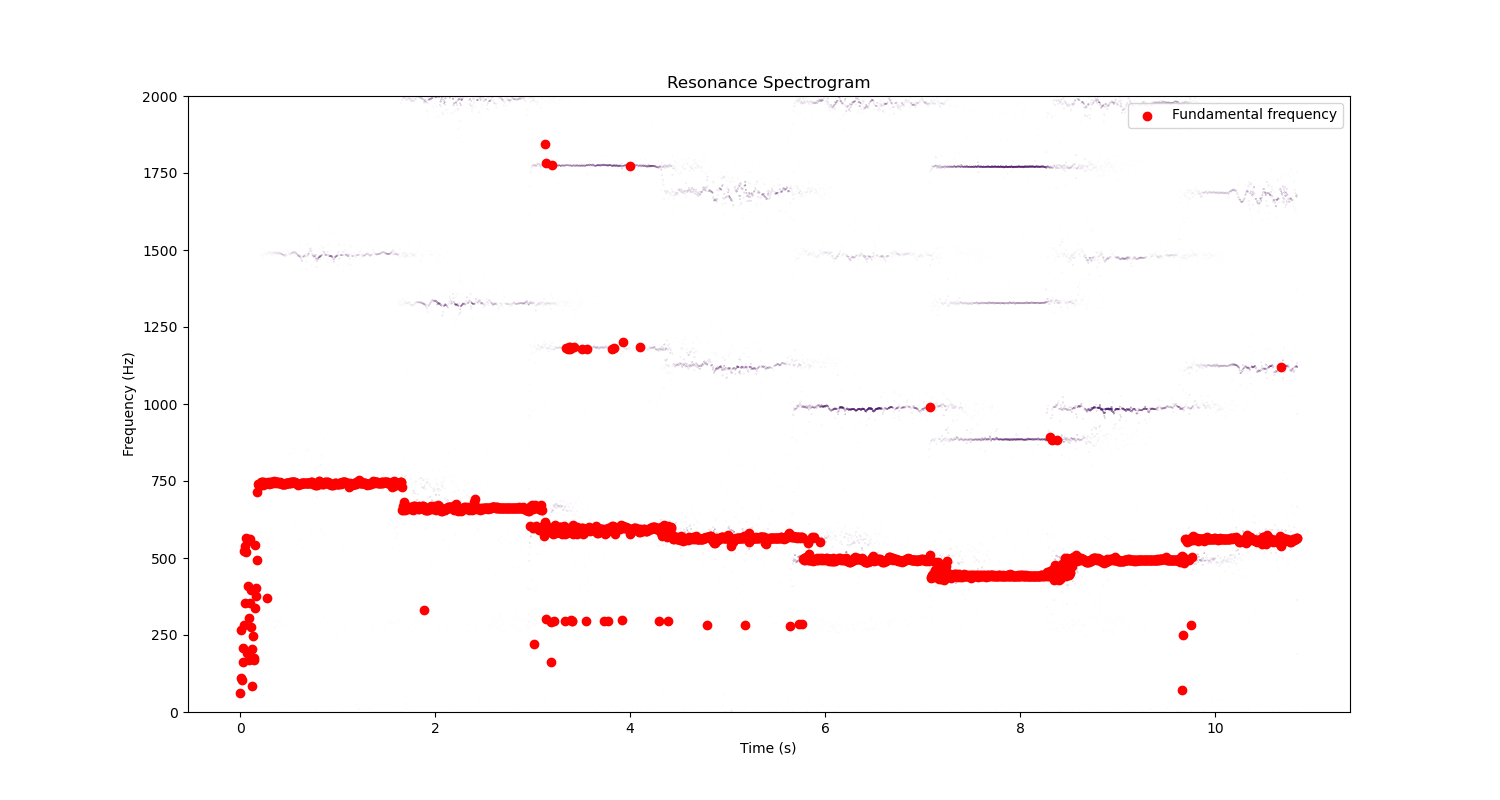
\includegraphics[width=1\linewidth]{images/cluster/violin_canonD_1_f0.png}
\caption{A slice (the first two measures) from a real audio recording of a violin performing \textit{Canon in D}, by Johann Pachelbel. Resonances that are estimated to belong to tonic root are highlighted in red.}
\label{rameauFundamental} 
\end{marginfigure}
As discussed earlier, musical instruments do not generate perfect sinusoidal waves. The reverberation of the sound in the environment, unique construction of the instrument, the inimitable single performance of a musician as well as the quality of recording equipment all contribute to the unique sound we capture in an audio recording. Noise, as well as harmonic and non-harmonic tones, interfere with each other, which makes the analysis of music relatively complex. 
Since humans perceive harmonics as a combination of overtones in harmonic series, we modelled the pitch perception by estimating the fundamental by the frequencies with the greatest relative harmonicity (Figure \ref{rameauFundamental}). Harmonicity refers to the distribution of power in a resonance, and since harmonic overtones are integer multiples of a fundamental tone, it is possible to estimate the fundamental, even in cases that the fundamental is missing, as was described in Chapter \ref{chap:Psychoacoustics} Psychoacoustics. For example, if a flute is playing an A4, the relative harmonicity with respect to A4 will be larger than the harmonicity of B4. The measurement of the relative harmonicity is examined through a resonance-harmonic inner product, described by \textcite{homer_modelling_2023} and defined as cosine similarity:

\begin{equation} 
S_C\left(f, H g_\eta-g_\eta\right)=\cos \theta=\frac{\operatorname{Re}\left[\left\langle f \mid H g_\eta-g_\eta\right\rangle\right]}{\|f\| \cdot\left\|H g_\eta-g_\eta\right\|}
\end{equation}

The fundamental frequency $\eta_0=\underset{\eta}{\arg \max }\left[S_C\left(f, H g_\eta-g_\eta\right)\right]$, which exactly estimates the frequencies with the greatest relative harmonicity.
\textcite{homer_modelling_2023} are also engaged in refining a method called the Rameau fundamental \sidenotemark\sidenotetext{Jean-Philippe \textcite{rameau_traite_1722} founded the modern musical theory with the publication \textit{Traité de l'harmonie réduite à ses principes naturels}, by mathematically proving that every pitch consists of a harmony. Rameau believed that the rules of harmony were derived from nature, called \textit{The vibrating world}, and these rules governed all music.}, which can currently be used for the Tonic root estimation, but should be further elaborated for recordings containing different instruments.


\section{Clustering}

\begin{marginfigure}
\centering
\vspace{1cm}
\includesvg[pretex=\fontsize{3pt}{5pt},width=1\linewidth]{images/cluster/e01pts4.svg}
\caption{$\epsilon$=0.1, minPts=4.}
\label{a} 
\end{marginfigure}


\begin{marginfigure}
\centering
\vspace{0.3cm}
\includesvg[pretex=\fontsize{3pt}{5pt},width=1\linewidth]{images/cluster/e01pts10.svg}
\caption{$\epsilon$=0.1, minPts=10.}
\label{b} 
\end{marginfigure}

\begin{marginfigure}
\centering
\vspace{0.3cm}
\includesvg[pretex=\fontsize{3pt}{5pt},width=1\linewidth]{images/cluster/e03pts4.svg}
\caption{$\epsilon$=0.3, minPts=10.}
\label{c} 
\end{marginfigure}





We performed the DBSCAN algorithm (discussed in Chapter \ref{chap:cluster}) on the detected fundamental frequencies in terms of frequency and onset to group resonances belonging to a certain note. In a slice (the first two measures) of a real audio recording of a violin performing \textit{Canon in D}, by Johann Pachelbel (\cite{bridget_stringspace_2019}), the DBSCAN algorithm has been performed with variable values of $\epsilon$ and $minPts$. Frequencies labeled with 0 are removed from the Figure \ref{clusteringRoot} and refer to all non-clustered resonances extracted from the audio file, frequencies labeled as -1 are labeled as noise from the Fundamental Frequency detection algorithm. 

\begin{figure}[h]
\centering
\includesvg[pretex=\fontsize{4pt}{6pt},width=0.9\linewidth]{images/applications/canonD.svg}
\vspace{0.1cm}
\caption{A correct labeling with the DBSCAN through correct parameter estimation. Performed on the first two measures of Canon in D.}
\label{clusteringRoot} 
\end{figure}

\subsection{Parameter estimation}

As mentioned earlier, $\epsilon$ and \textit{minPts} are the two parameters to be estimated. Variations in clustering when varying the two parameters are represented in Figures \ref{a}-\ref{c}. Therefore, we will introduce two automatic parameter estimators: the silhouette score and \textit{kneedle} method.


\subsubsection{Silhouette Score}
The silhouette score is a normalized metric for the evaluation of the quality of a clustering technique:

\begin{equation}
\text{silhouette score} = \frac{\beta-\alpha}{\max(\alpha,\beta)}.
\end{equation}

$\alpha$ denotes the average distance between the points inside a cluster, and $\beta$ the average distance between all clusters. A high positive value implies that the clusters are will distinct from one another, indicating a good clustering performance. Values close to 0 imply cluster overlapping, and negative scores tending towards -1 imply wrongly assigned points (\cite{rousseeuw_silhouettes_1987}).

\subsubsection{Kneedle Method}


Several methods exist to estimate an optimal value for $\epsilon$. Satopaa proposed the knee method in \textit{"Finding a "Kneedle" in a Haystack: Detecting Knee Points in System Behavior"} (\cite{satopaa_finding_2011}). From a k-distance graph, with values sorted from small to large (or vice versa), the optimal parameters can graphically be estimated by finding a knee or elbow in the graph as illustrated in Figure \ref{fig:kneedle}. 
The mathematical definition of the curvature is the basis definition for the knee estimate. \textcite{satopaa_finding_2011} defined the Kneedle-algorithm as following:

\begin{marginfigure}
\vspace{2cm}
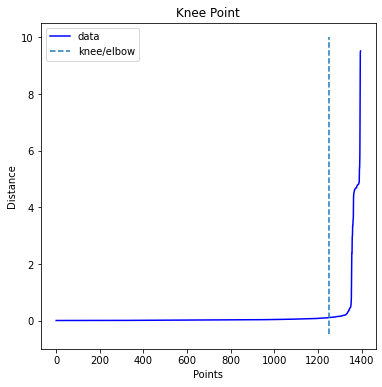
\includegraphics[width=1\linewidth]{images/cluster/kneePoint.png}
\caption{Kneedle of a harmonic series from C5 to F played by a flute.}
\label{fig:kneedle} 
\end{marginfigure}

\begin{definition}[Kneedle]
For a continuous function $f$, there exists a $K_f(x)$ that defines the curvature of $f$ at any point as a function of its first and second derivative:
\begin{equation}
K_f(x)=\frac{f^{\prime \prime}(x)}{\left(1+f^{\prime}(x)^2\right)^{1.5}}.
\end{equation}
\end{definition}

The point of maximum curvature is used in the Kneedle-algorithm to select the optimal value for $\epsilon$, which is (1 - normalized value) of the knee locator (or just the normalized value if inverse density ordering was implemented). It is worth mentioning that the clustering results are significantly impacted by the choice of $\epsilon$. A small value of $\epsilon$ will lead to inadequate clustering, whereas a high value will result in most objects being merged into a single cluster.


\subsection{Clustering Performance Evaluation}

The rule of thumb for a threshold value of the minimum amount of neighbors within a radius $\epsilon$, is \textit{minPts} = dim$*2$ (\cite{ester_density-based_1996, sander_density-based_1998}). However, if the dataset is large or contains noisy data, a larger value for \textit{minPts} can be required. The threshold value was therefore estimated with the silhouette score and a method comparison study for the $\epsilon$-estimation was performed to evaluate the difference between the Kneedle-algorithm and silhouette score on the quality of clustering. We examined the detection of 159 synthetically generated notes. The evaluated notes differ in duration, pitch and distance. The hit or miss criterion was based on whether a group of resonances representing a note was detected or not. We noticed that the silhouette score performed a significantly better clustering than the \textit{kneedle} method. However, in both methods, due to the not-yet-perfect $f_0$ estimation, noise was clustered together and influences the results. 

\subsection{Clusters of noise} 
In this specific section, when we mention \textit{noise}, we are referring to resonances that are detected along with the fundamental tone, even though they are not actually part of it. Most of them are classified as -1 by the DBSCAN algorithm, but closely laying noisy points form sometimes unwanted little clusters of overtones. However, they mostly have a relatively low power compared to the resonances presented in the real fundamental. 
Therefore, we removed the clusters containing a significantly lower power on average. The difference between a plot with and without power is shown in Figure \ref{remove_lowpower}. It is crucial to get rid of these clusters of noise for attributing constituents to a particular note in our system, as well as for the musical transcription of the sound.

\begin{figure}[h]
\centering
\includesvg[pretex=\fontsize{4pt}{6pt},width=1\linewidth]{images/cluster/remove_lowpower.svg}
\caption{A comparison between two three-dimensional plots with a third axis denoting the power. Clusters with a small average power, relative to the other ones, are removed.}
\label{remove_lowpower} 
\end{figure}



\section{Attributing a Note Constituent}
Resonances belonging to a cluster are each assigned to a constituent representing a musical \textit{note}, attributed with the average frequency, onset, off-set and relative duration. Extracting the real rhythm of a live performance is more complicated than it seems, since people never play perfectly on the beat as written on paper. Therefore, we focused on the accurate extraction of pitch for this thesis, and suggested a relative estimation of the duration in our software. It correctly estimates the duration of notes for computer-generated audio files, but needs a refinement for audio files performed by humans in future work. 


\subsubsection{Example: Syrinx (Flute Solo)}
\begin{figure}[h]
\centering
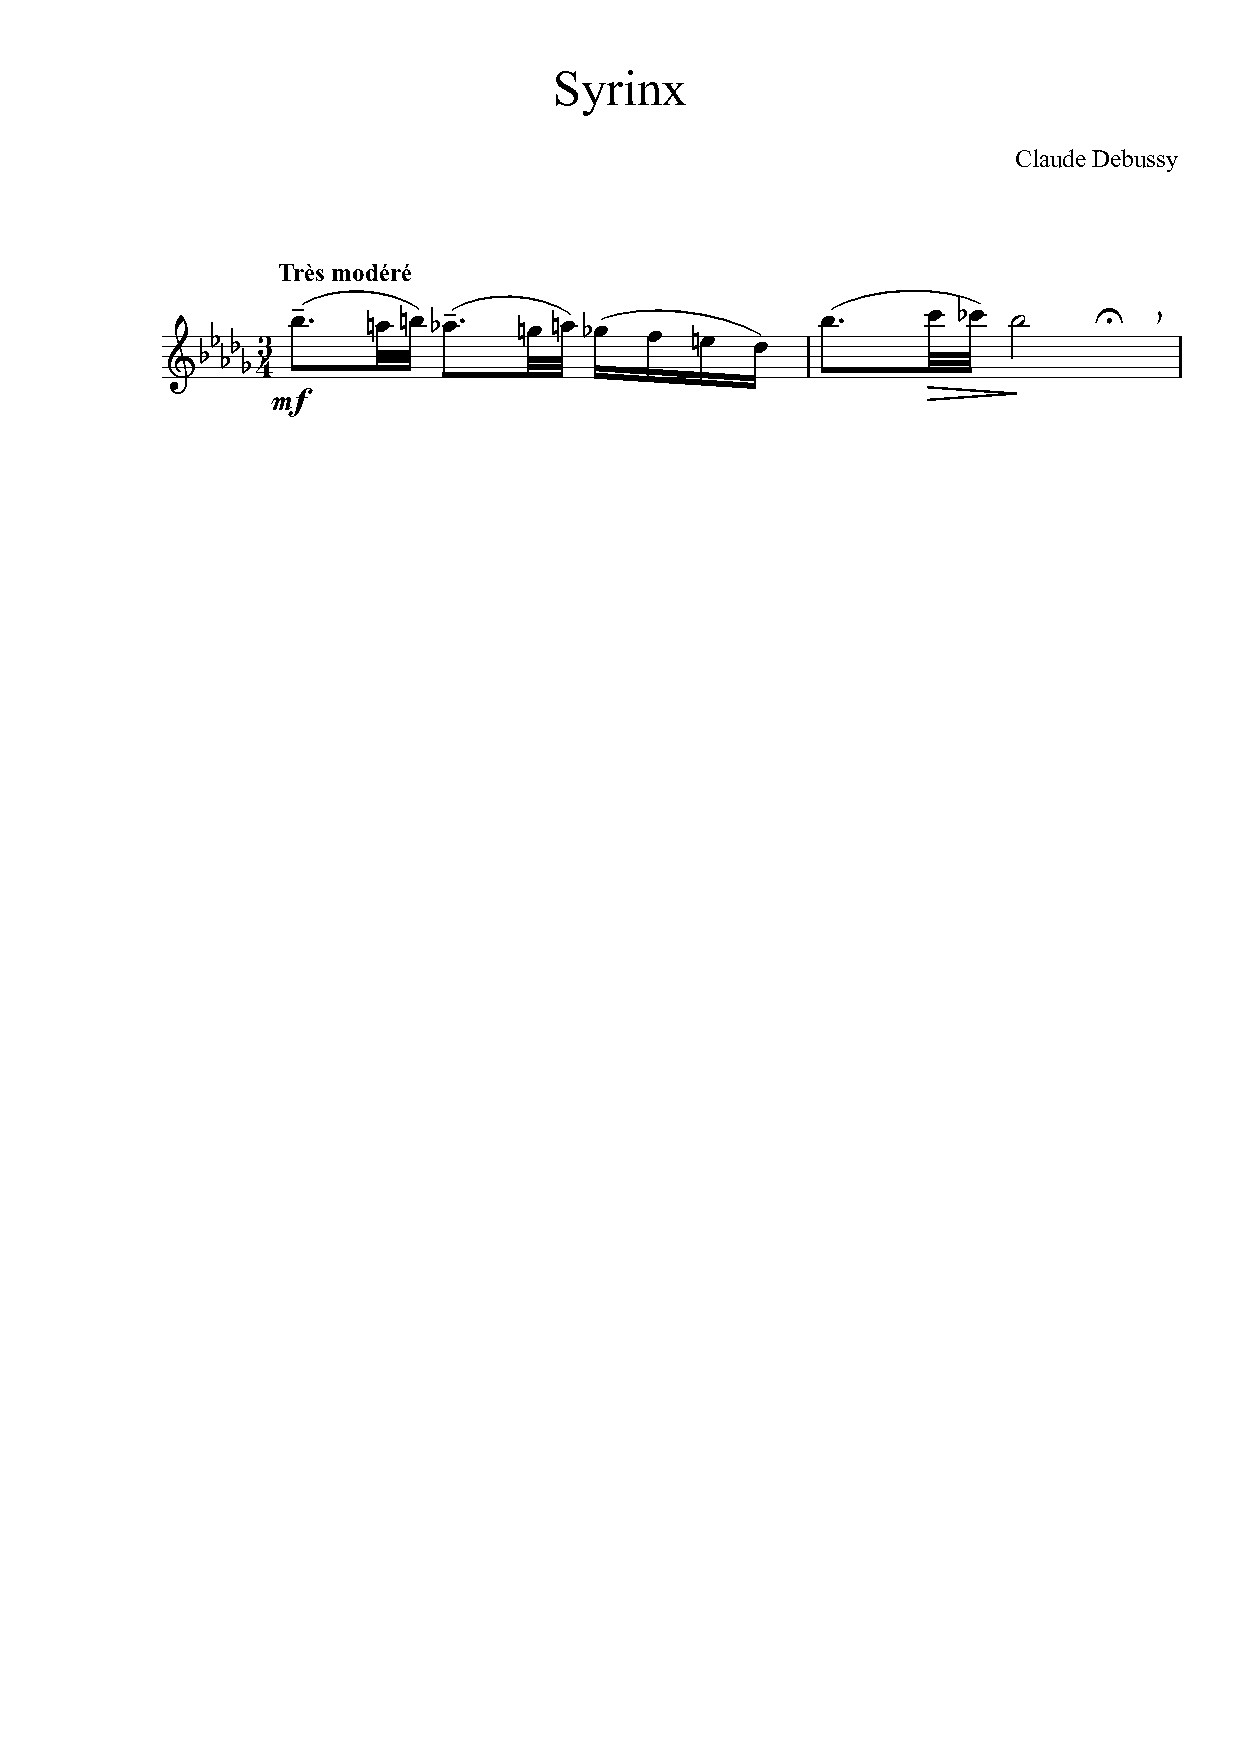
\includegraphics[width=1\linewidth]{images/applications/syrinx_original.pdf}
\caption{Western score notation of the first two measures of Syrinx, by Claude Debussy.}
\label{syrinx_original} 
\end{figure}
We analyzed the pitch estimation of a slice of \textit{Syrinx}, by Claude Debussy, performed by a real and artificially generated flute. The ground truth music score is presented in Figure \ref{syrinx_original}.
The first two measures have strong variations in rhythm and the notes are laying nearby, which makes is harder for the cluster algorithm to recognize two different objects. With the application of our method on this sample, the pitch of each note was correctly reconstructed based on the frequency data within each cluster. Please note that there is a slight difference in notation due to the key signature in the original piece. Thus, the pitch of each note in this slice has been assigned correctly\sidenotemark\sidenotetext{About musical notation: The flat ($\flat$), sharp ($\sharp$), and natural ($\natural$) signs preceding a note indicate that the note should be played a semitone lower, higher, or disregarding the sign in the key signature or the modification of a tone within the same measure.}, as illustrated in Figure \ref{syrinx_artificial}.


\begin{figure}[h]
\centering
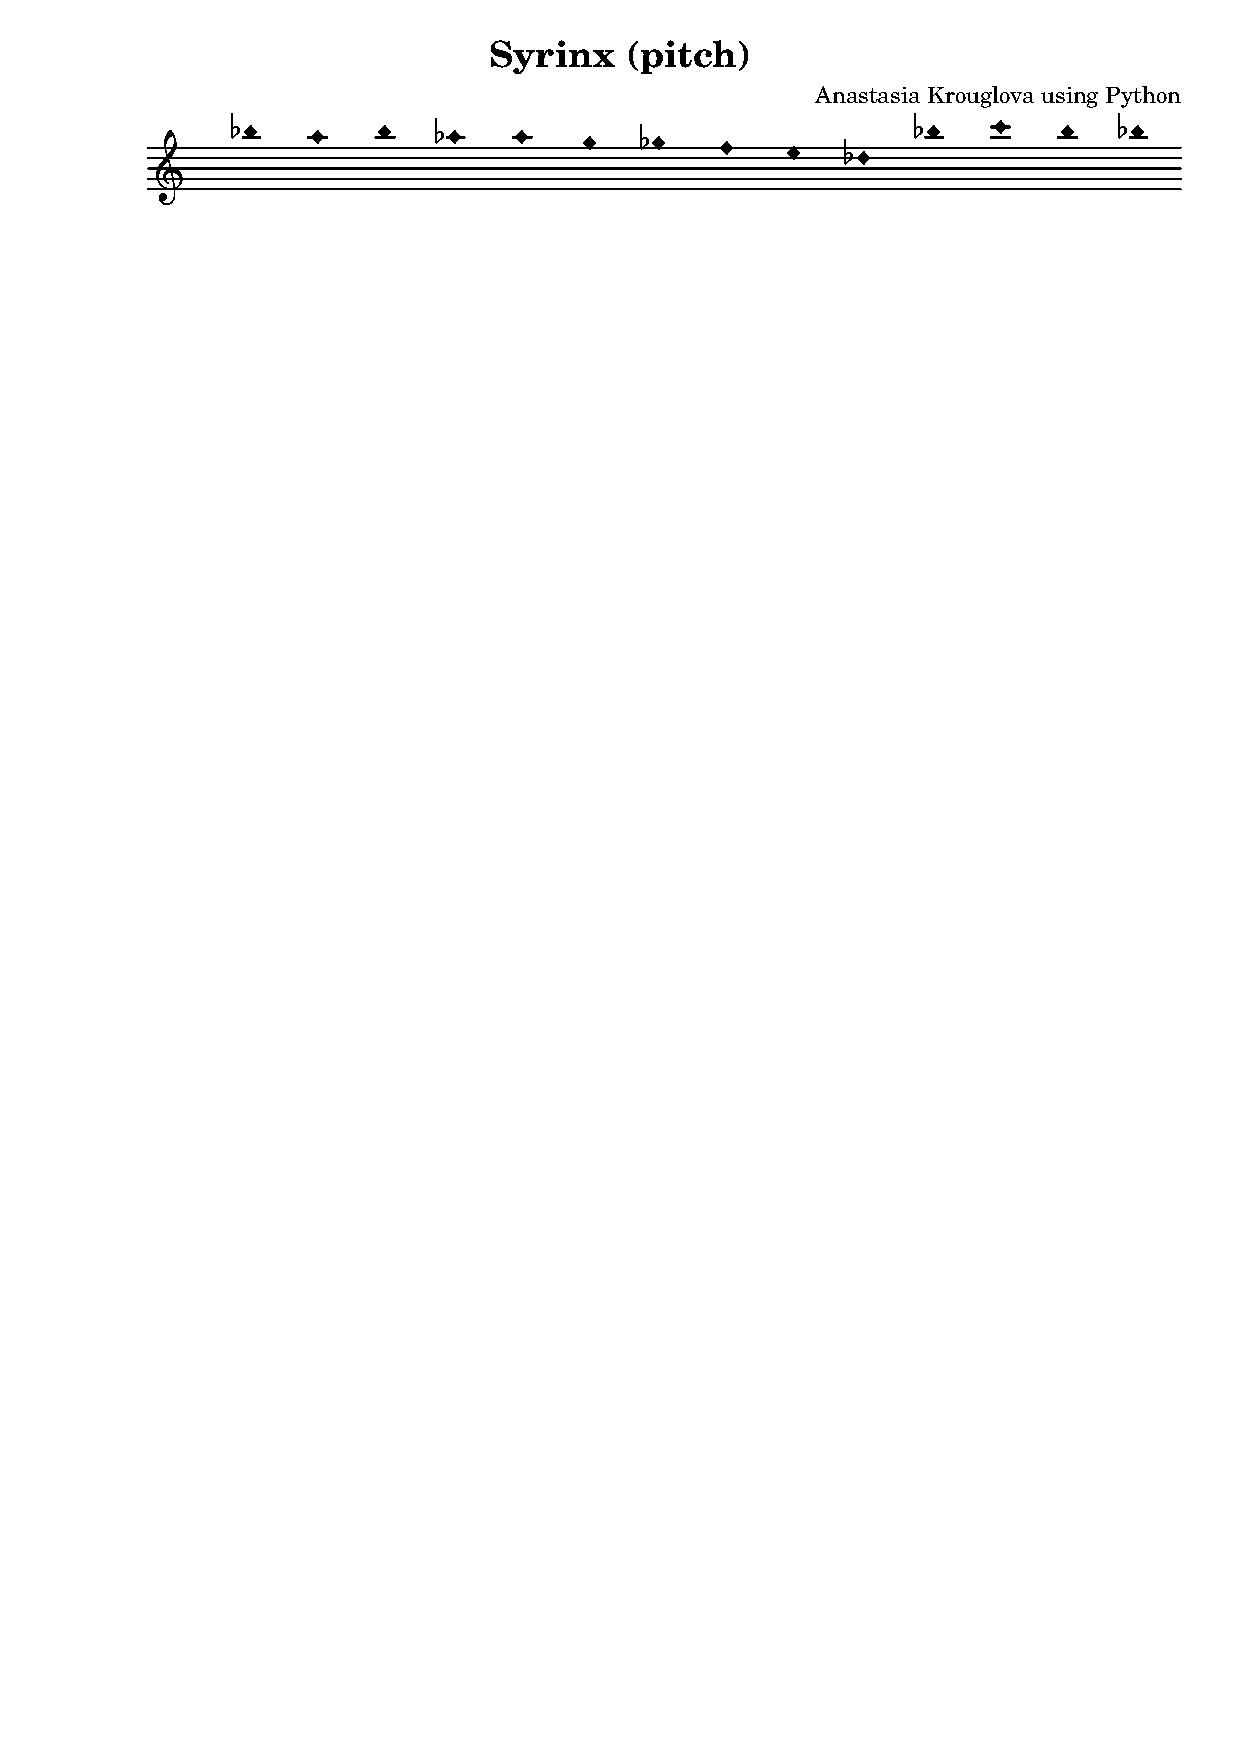
\includegraphics[width=0.9\linewidth]{images/applications/pitches_syrinx.pdf}
\caption{The pitches in the first measure of Syrinx, by Claude Debussy were correctly assigned and serve as one of the attributes for the Note constituent.}
\label{syrinx_artificial} 
\end{figure}

\begin{marginfigure}
\centering
\vspace{1.8cm}
\includesvg[pretex=\fontsize{6pt}{8pt}, width=1\linewidth]{images/applications/harm.svg}
\vspace{0.1cm}
\caption{The hierarchy of harmonics is part of the Frame-level description of music, highlighted in purple.}
\label{harmonyExtraction} 
\end{marginfigure}


\section{Towards a Frame-level description}
We introduce our approach towards a subtask of the frame-level description of music, namely the extractions of harmonic overtones. The frame-level description (i.e., multi-pitch estimation) estimates the number of notes that are simultaneously played in a slice of time (\cite{benetos_automatic_2019}). It is currently based on the assumption that the fundamental tone is known, but should be expanded to a relative estimation and extraction of overtones for polyphonic music.


\subsection{Attributing the Harmonic Constituent}
As discussed in the chapter about psychoacoustics, a real musical tone often consists of a fundamental, but also from harmonic and non-harmonic overtones. Since harmonic overtones are integer multiples of the fundamental tones, they can be found by defining them in a space of the so-called $f_0$-likeliness ($H$):

\begin{equation}
    H = E(\frac{f}{f_0} \mod{1})
\end{equation}

\begin{marginfigure}
\centering
\includesvg[pretex=\fontsize{3.3pt}{5pt}, width=1.12\linewidth]{images/cluster/canonD_overtones.svg}
\vspace{0.1cm}
\caption{The extraction of the harmonic overtone from a real audio recording performed by \textcite{bridget_stringspace_2019} (produced and approved for use by Stringspace).}
\label{overtonesPlot} 
\end{marginfigure}



$E \sim \mathcal{N}(0.5, 0.5)$ simulates the idea of entropy for the definition of how likely a resonance is part of an overtone.
We used a real audio recording of a violin performing Canon in D, by Johann Pachelbel (\cite{bridget_stringspace_2019}) to analyze the overtones of a violin. We limited the space with a bound defined in the $H$ space, which give us a first approximation of the overtones if the fundamental is known.
    
    \chapter*{Conclusion}
\label{ch:conclusion}
\addcontentsline{toc}{chapter}{\nameref{ch:conclusion}}


% SUMMARIZE RESEARCH OBJECTIVES
The aim of this thesis was to create a multipurpose cognitive framework for musical analysis. 
% RECAP METHODOLOGY
We modelled human-like perception with the discrete resonance spectrum, grouped this information with cognitive models and structured the clusters in a type-based knowledge representation.
% RECAP FOUND
We extracted musical structures from audio files and stored them in a hierarchical structure. This way, a bidirectional link between knowledge and data was obtained.
% SIGNIFICANCE
Our methodology allows us to infer knowledge from different methods and build a system for a long-term perspective. 
% MY CONTRIBUTION
Moreover, by using a cognitive clustering-approach, one of the fundamental music transcription challenges of overlapping tones has been resolved.
% CONCLUSION
To conclude, we created a tool that gives a range of possibilities in different subtasks of musical analysis and can push this research domain further by allowing inference between various machine learning models.
    \chapter*{Further Work}
\label{ch:furtherWork}
\addcontentsline{toc}{chapter}{\nameref{ch:furtherWork}}


For future work, we suggest to search for a cognitive approach towards a multi-pitch estimation of music, since the inference of musical attributes, such as pitch, in a polyphonic musical signal is a highly challenging problem (\cite{benetos_automatic_2019}). Further, we also propose to improve the relative estimation of note durations which is currently present in our software, for a more accurate musical transcription of musical signals. It would also be interesting to extract less mainstream musical structures, such as phrases. For instance, they can be perceived as a musician gently inhaling before playing wind instruments, the subtle shift in bow direction for string instruments, or the relative power of notes in key instruments.

    % appendix
    \chapter*{Nomenclature}
\label{ch:nomenclature}
\addcontentsline{toc}{chapter}{\nameref{ch:nomenclature}}


\section*{Symbols}
\begin{tabbing}
 \hspace*{1.6cm} \= \hspace*{8cm} \= \kill
 $d_k$ \> Initial complex amplitude of a resonance  \\[0.5ex]
 $\psi_k$ \> Initial phase of a resonance  \\[0.5ex]
 $\phi_k$ \> Real frequency of the resonance \\[0.5ex]
$\omega_k$ \> Complex frequency of a resonance ($\phi_k+ i\gamma_k$) \\[0.5ex]
$\gamma_k$ \> Rate of decay \\[0.5ex]
$\mathcal {F}[f(t)]$ \> Fourier transform of a time-domain signal  \\[0.5ex]
$\mathcal {F}^{-1}[\hat{f}(\omega)]$ \> Inverse Fourier transform of a frequency-domain signal  \\[0.5ex]

$|| f ||$ \> Norm of $f$  \\[0.5ex]
$\braket{\alpha | \beta}$ \> Inner product  \\[0.5ex]
$\overline{f(x)}$ \> Complex conjugate  \\[0.5ex]
$P(i)$ \> Particles of a Constituent  \\[0.5ex]
$R(i)$ \> Attributes of a Constituent  \\[0.5ex]

  
\end{tabbing}
\section*{Acronyms and Abbreviations}
\begin{tabbing}
 \hspace*{1.6cm}  \= \kill

    Cic \> Calculus of Inductive Constructions \\[0.5ex]
Coq \>  library with Calculus of Inductive Constructions as underlying
formal language \\[0.5ex]
 CSPEC \> Type of constituent specifications \\[0.5ex]
  CHAKRA \> Common Hierarchical Abstract Knowledge Representation for Anything \\[0.5ex]
 CHARM \> Common Hierarchical Abstract Representation of Music \\[0.5ex]
  DAG \> Directed Acyclic Graph \\[0.5ex]
 DBSCAN \> Density-based spatial clustering of applications with noise \\[0.5ex]
  DFT \> Discrete Fourier Transform \\[0.5ex]
  FFT \> Fast Fourier Transform \\[0.5ex]
  $L^2$ \> Space of absolutely square-summable functions \\[0.5ex]
  STFT \> Short Time Fourier Transform \\[0.5ex]
VUB \> Vrije Universiteit Brussel \\[0.5ex]




\end{tabbing}





   
    \printbibliography
\end{document}
